\documentclass[11pt]{article}

    \usepackage[breakable]{tcolorbox}
    \usepackage{parskip} % Stop auto-indenting (to mimic markdown behaviour)
    
    \usepackage{iftex}
    \ifPDFTeX
    	\usepackage[T1]{fontenc}
    	\usepackage{mathpazo}
    \else
    	\usepackage{fontspec}
    \fi

    % Basic figure setup, for now with no caption control since it's done
    % automatically by Pandoc (which extracts ![](path) syntax from Markdown).
    \usepackage{graphicx}
    % Maintain compatibility with old templates. Remove in nbconvert 6.0
    \let\Oldincludegraphics\includegraphics
    % Ensure that by default, figures have no caption (until we provide a
    % proper Figure object with a Caption API and a way to capture that
    % in the conversion process - todo).
    \usepackage{caption}
    \DeclareCaptionFormat{nocaption}{}
    \captionsetup{format=nocaption,aboveskip=0pt,belowskip=0pt}

    \usepackage{float}
    \floatplacement{figure}{H} % forces figures to be placed at the correct location
    \usepackage{xcolor} % Allow colors to be defined
    \usepackage{enumerate} % Needed for markdown enumerations to work
    \usepackage{geometry} % Used to adjust the document margins
    \usepackage{amsmath} % Equations
    \usepackage{amssymb} % Equations
    \usepackage{textcomp} % defines textquotesingle
    % Hack from http://tex.stackexchange.com/a/47451/13684:
    \AtBeginDocument{%
        \def\PYZsq{\textquotesingle}% Upright quotes in Pygmentized code
    }
    \usepackage{upquote} % Upright quotes for verbatim code
    \usepackage{eurosym} % defines \euro
    \usepackage[mathletters]{ucs} % Extended unicode (utf-8) support
    \usepackage{fancyvrb} % verbatim replacement that allows latex
    \usepackage{grffile} % extends the file name processing of package graphics 
                         % to support a larger range
    \makeatletter % fix for old versions of grffile with XeLaTeX
    \@ifpackagelater{grffile}{2019/11/01}
    {
      % Do nothing on new versions
    }
    {
      \def\Gread@@xetex#1{%
        \IfFileExists{"\Gin@base".bb}%
        {\Gread@eps{\Gin@base.bb}}%
        {\Gread@@xetex@aux#1}%
      }
    }
    \makeatother
    \usepackage[Export]{adjustbox} % Used to constrain images to a maximum size
    \adjustboxset{max size={0.9\linewidth}{0.9\paperheight}}

    % The hyperref package gives us a pdf with properly built
    % internal navigation ('pdf bookmarks' for the table of contents,
    % internal cross-reference links, web links for URLs, etc.)
    \usepackage{hyperref}
    % The default LaTeX title has an obnoxious amount of whitespace. By default,
    % titling removes some of it. It also provides customization options.
    \usepackage{titling}
    \usepackage{longtable} % longtable support required by pandoc >1.10
    \usepackage{booktabs}  % table support for pandoc > 1.12.2
    \usepackage[inline]{enumitem} % IRkernel/repr support (it uses the enumerate* environment)
    \usepackage[normalem]{ulem} % ulem is needed to support strikethroughs (\sout)
                                % normalem makes italics be italics, not underlines
    \usepackage{mathrsfs}
    

    
    % Colors for the hyperref package
    \definecolor{urlcolor}{rgb}{0,.145,.698}
    \definecolor{linkcolor}{rgb}{.71,0.21,0.01}
    \definecolor{citecolor}{rgb}{.12,.54,.11}

    % ANSI colors
    \definecolor{ansi-black}{HTML}{3E424D}
    \definecolor{ansi-black-intense}{HTML}{282C36}
    \definecolor{ansi-red}{HTML}{E75C58}
    \definecolor{ansi-red-intense}{HTML}{B22B31}
    \definecolor{ansi-green}{HTML}{00A250}
    \definecolor{ansi-green-intense}{HTML}{007427}
    \definecolor{ansi-yellow}{HTML}{DDB62B}
    \definecolor{ansi-yellow-intense}{HTML}{B27D12}
    \definecolor{ansi-blue}{HTML}{208FFB}
    \definecolor{ansi-blue-intense}{HTML}{0065CA}
    \definecolor{ansi-magenta}{HTML}{D160C4}
    \definecolor{ansi-magenta-intense}{HTML}{A03196}
    \definecolor{ansi-cyan}{HTML}{60C6C8}
    \definecolor{ansi-cyan-intense}{HTML}{258F8F}
    \definecolor{ansi-white}{HTML}{C5C1B4}
    \definecolor{ansi-white-intense}{HTML}{A1A6B2}
    \definecolor{ansi-default-inverse-fg}{HTML}{FFFFFF}
    \definecolor{ansi-default-inverse-bg}{HTML}{000000}

    % common color for the border for error outputs.
    \definecolor{outerrorbackground}{HTML}{FFDFDF}

    % commands and environments needed by pandoc snippets
    % extracted from the output of `pandoc -s`
    \providecommand{\tightlist}{%
      \setlength{\itemsep}{0pt}\setlength{\parskip}{0pt}}
    \DefineVerbatimEnvironment{Highlighting}{Verbatim}{commandchars=\\\{\}}
    % Add ',fontsize=\small' for more characters per line
    \newenvironment{Shaded}{}{}
    \newcommand{\KeywordTok}[1]{\textcolor[rgb]{0.00,0.44,0.13}{\textbf{{#1}}}}
    \newcommand{\DataTypeTok}[1]{\textcolor[rgb]{0.56,0.13,0.00}{{#1}}}
    \newcommand{\DecValTok}[1]{\textcolor[rgb]{0.25,0.63,0.44}{{#1}}}
    \newcommand{\BaseNTok}[1]{\textcolor[rgb]{0.25,0.63,0.44}{{#1}}}
    \newcommand{\FloatTok}[1]{\textcolor[rgb]{0.25,0.63,0.44}{{#1}}}
    \newcommand{\CharTok}[1]{\textcolor[rgb]{0.25,0.44,0.63}{{#1}}}
    \newcommand{\StringTok}[1]{\textcolor[rgb]{0.25,0.44,0.63}{{#1}}}
    \newcommand{\CommentTok}[1]{\textcolor[rgb]{0.38,0.63,0.69}{\textit{{#1}}}}
    \newcommand{\OtherTok}[1]{\textcolor[rgb]{0.00,0.44,0.13}{{#1}}}
    \newcommand{\AlertTok}[1]{\textcolor[rgb]{1.00,0.00,0.00}{\textbf{{#1}}}}
    \newcommand{\FunctionTok}[1]{\textcolor[rgb]{0.02,0.16,0.49}{{#1}}}
    \newcommand{\RegionMarkerTok}[1]{{#1}}
    \newcommand{\ErrorTok}[1]{\textcolor[rgb]{1.00,0.00,0.00}{\textbf{{#1}}}}
    \newcommand{\NormalTok}[1]{{#1}}
    
    % Additional commands for more recent versions of Pandoc
    \newcommand{\ConstantTok}[1]{\textcolor[rgb]{0.53,0.00,0.00}{{#1}}}
    \newcommand{\SpecialCharTok}[1]{\textcolor[rgb]{0.25,0.44,0.63}{{#1}}}
    \newcommand{\VerbatimStringTok}[1]{\textcolor[rgb]{0.25,0.44,0.63}{{#1}}}
    \newcommand{\SpecialStringTok}[1]{\textcolor[rgb]{0.73,0.40,0.53}{{#1}}}
    \newcommand{\ImportTok}[1]{{#1}}
    \newcommand{\DocumentationTok}[1]{\textcolor[rgb]{0.73,0.13,0.13}{\textit{{#1}}}}
    \newcommand{\AnnotationTok}[1]{\textcolor[rgb]{0.38,0.63,0.69}{\textbf{\textit{{#1}}}}}
    \newcommand{\CommentVarTok}[1]{\textcolor[rgb]{0.38,0.63,0.69}{\textbf{\textit{{#1}}}}}
    \newcommand{\VariableTok}[1]{\textcolor[rgb]{0.10,0.09,0.49}{{#1}}}
    \newcommand{\ControlFlowTok}[1]{\textcolor[rgb]{0.00,0.44,0.13}{\textbf{{#1}}}}
    \newcommand{\OperatorTok}[1]{\textcolor[rgb]{0.40,0.40,0.40}{{#1}}}
    \newcommand{\BuiltInTok}[1]{{#1}}
    \newcommand{\ExtensionTok}[1]{{#1}}
    \newcommand{\PreprocessorTok}[1]{\textcolor[rgb]{0.74,0.48,0.00}{{#1}}}
    \newcommand{\AttributeTok}[1]{\textcolor[rgb]{0.49,0.56,0.16}{{#1}}}
    \newcommand{\InformationTok}[1]{\textcolor[rgb]{0.38,0.63,0.69}{\textbf{\textit{{#1}}}}}
    \newcommand{\WarningTok}[1]{\textcolor[rgb]{0.38,0.63,0.69}{\textbf{\textit{{#1}}}}}
    
    
    % Define a nice break command that doesn't care if a line doesn't already
    % exist.
    \def\br{\hspace*{\fill} \\* }
    % Math Jax compatibility definitions
    \def\gt{>}
    \def\lt{<}
    \let\Oldtex\TeX
    \let\Oldlatex\LaTeX
    \renewcommand{\TeX}{\textrm{\Oldtex}}
    \renewcommand{\LaTeX}{\textrm{\Oldlatex}}
    % Document parameters
    % Document title
    \title{Traffic}
    
    
    
    \author{Nicola Ronzoni: Intern at Inria, ACUMES team}
    
    
    
% Pygments definitions
\makeatletter
\def\PY@reset{\let\PY@it=\relax \let\PY@bf=\relax%
    \let\PY@ul=\relax \let\PY@tc=\relax%
    \let\PY@bc=\relax \let\PY@ff=\relax}
\def\PY@tok#1{\csname PY@tok@#1\endcsname}
\def\PY@toks#1+{\ifx\relax#1\empty\else%
    \PY@tok{#1}\expandafter\PY@toks\fi}
\def\PY@do#1{\PY@bc{\PY@tc{\PY@ul{%
    \PY@it{\PY@bf{\PY@ff{#1}}}}}}}
\def\PY#1#2{\PY@reset\PY@toks#1+\relax+\PY@do{#2}}

\expandafter\def\csname PY@tok@w\endcsname{\def\PY@tc##1{\textcolor[rgb]{0.73,0.73,0.73}{##1}}}
\expandafter\def\csname PY@tok@c\endcsname{\let\PY@it=\textit\def\PY@tc##1{\textcolor[rgb]{0.25,0.50,0.50}{##1}}}
\expandafter\def\csname PY@tok@cp\endcsname{\def\PY@tc##1{\textcolor[rgb]{0.74,0.48,0.00}{##1}}}
\expandafter\def\csname PY@tok@k\endcsname{\let\PY@bf=\textbf\def\PY@tc##1{\textcolor[rgb]{0.00,0.50,0.00}{##1}}}
\expandafter\def\csname PY@tok@kp\endcsname{\def\PY@tc##1{\textcolor[rgb]{0.00,0.50,0.00}{##1}}}
\expandafter\def\csname PY@tok@kt\endcsname{\def\PY@tc##1{\textcolor[rgb]{0.69,0.00,0.25}{##1}}}
\expandafter\def\csname PY@tok@o\endcsname{\def\PY@tc##1{\textcolor[rgb]{0.40,0.40,0.40}{##1}}}
\expandafter\def\csname PY@tok@ow\endcsname{\let\PY@bf=\textbf\def\PY@tc##1{\textcolor[rgb]{0.67,0.13,1.00}{##1}}}
\expandafter\def\csname PY@tok@nb\endcsname{\def\PY@tc##1{\textcolor[rgb]{0.00,0.50,0.00}{##1}}}
\expandafter\def\csname PY@tok@nf\endcsname{\def\PY@tc##1{\textcolor[rgb]{0.00,0.00,1.00}{##1}}}
\expandafter\def\csname PY@tok@nc\endcsname{\let\PY@bf=\textbf\def\PY@tc##1{\textcolor[rgb]{0.00,0.00,1.00}{##1}}}
\expandafter\def\csname PY@tok@nn\endcsname{\let\PY@bf=\textbf\def\PY@tc##1{\textcolor[rgb]{0.00,0.00,1.00}{##1}}}
\expandafter\def\csname PY@tok@ne\endcsname{\let\PY@bf=\textbf\def\PY@tc##1{\textcolor[rgb]{0.82,0.25,0.23}{##1}}}
\expandafter\def\csname PY@tok@nv\endcsname{\def\PY@tc##1{\textcolor[rgb]{0.10,0.09,0.49}{##1}}}
\expandafter\def\csname PY@tok@no\endcsname{\def\PY@tc##1{\textcolor[rgb]{0.53,0.00,0.00}{##1}}}
\expandafter\def\csname PY@tok@nl\endcsname{\def\PY@tc##1{\textcolor[rgb]{0.63,0.63,0.00}{##1}}}
\expandafter\def\csname PY@tok@ni\endcsname{\let\PY@bf=\textbf\def\PY@tc##1{\textcolor[rgb]{0.60,0.60,0.60}{##1}}}
\expandafter\def\csname PY@tok@na\endcsname{\def\PY@tc##1{\textcolor[rgb]{0.49,0.56,0.16}{##1}}}
\expandafter\def\csname PY@tok@nt\endcsname{\let\PY@bf=\textbf\def\PY@tc##1{\textcolor[rgb]{0.00,0.50,0.00}{##1}}}
\expandafter\def\csname PY@tok@nd\endcsname{\def\PY@tc##1{\textcolor[rgb]{0.67,0.13,1.00}{##1}}}
\expandafter\def\csname PY@tok@s\endcsname{\def\PY@tc##1{\textcolor[rgb]{0.73,0.13,0.13}{##1}}}
\expandafter\def\csname PY@tok@sd\endcsname{\let\PY@it=\textit\def\PY@tc##1{\textcolor[rgb]{0.73,0.13,0.13}{##1}}}
\expandafter\def\csname PY@tok@si\endcsname{\let\PY@bf=\textbf\def\PY@tc##1{\textcolor[rgb]{0.73,0.40,0.53}{##1}}}
\expandafter\def\csname PY@tok@se\endcsname{\let\PY@bf=\textbf\def\PY@tc##1{\textcolor[rgb]{0.73,0.40,0.13}{##1}}}
\expandafter\def\csname PY@tok@sr\endcsname{\def\PY@tc##1{\textcolor[rgb]{0.73,0.40,0.53}{##1}}}
\expandafter\def\csname PY@tok@ss\endcsname{\def\PY@tc##1{\textcolor[rgb]{0.10,0.09,0.49}{##1}}}
\expandafter\def\csname PY@tok@sx\endcsname{\def\PY@tc##1{\textcolor[rgb]{0.00,0.50,0.00}{##1}}}
\expandafter\def\csname PY@tok@m\endcsname{\def\PY@tc##1{\textcolor[rgb]{0.40,0.40,0.40}{##1}}}
\expandafter\def\csname PY@tok@gh\endcsname{\let\PY@bf=\textbf\def\PY@tc##1{\textcolor[rgb]{0.00,0.00,0.50}{##1}}}
\expandafter\def\csname PY@tok@gu\endcsname{\let\PY@bf=\textbf\def\PY@tc##1{\textcolor[rgb]{0.50,0.00,0.50}{##1}}}
\expandafter\def\csname PY@tok@gd\endcsname{\def\PY@tc##1{\textcolor[rgb]{0.63,0.00,0.00}{##1}}}
\expandafter\def\csname PY@tok@gi\endcsname{\def\PY@tc##1{\textcolor[rgb]{0.00,0.63,0.00}{##1}}}
\expandafter\def\csname PY@tok@gr\endcsname{\def\PY@tc##1{\textcolor[rgb]{1.00,0.00,0.00}{##1}}}
\expandafter\def\csname PY@tok@ge\endcsname{\let\PY@it=\textit}
\expandafter\def\csname PY@tok@gs\endcsname{\let\PY@bf=\textbf}
\expandafter\def\csname PY@tok@gp\endcsname{\let\PY@bf=\textbf\def\PY@tc##1{\textcolor[rgb]{0.00,0.00,0.50}{##1}}}
\expandafter\def\csname PY@tok@go\endcsname{\def\PY@tc##1{\textcolor[rgb]{0.53,0.53,0.53}{##1}}}
\expandafter\def\csname PY@tok@gt\endcsname{\def\PY@tc##1{\textcolor[rgb]{0.00,0.27,0.87}{##1}}}
\expandafter\def\csname PY@tok@err\endcsname{\def\PY@bc##1{\setlength{\fboxsep}{0pt}\fcolorbox[rgb]{1.00,0.00,0.00}{1,1,1}{\strut ##1}}}
\expandafter\def\csname PY@tok@kc\endcsname{\let\PY@bf=\textbf\def\PY@tc##1{\textcolor[rgb]{0.00,0.50,0.00}{##1}}}
\expandafter\def\csname PY@tok@kd\endcsname{\let\PY@bf=\textbf\def\PY@tc##1{\textcolor[rgb]{0.00,0.50,0.00}{##1}}}
\expandafter\def\csname PY@tok@kn\endcsname{\let\PY@bf=\textbf\def\PY@tc##1{\textcolor[rgb]{0.00,0.50,0.00}{##1}}}
\expandafter\def\csname PY@tok@kr\endcsname{\let\PY@bf=\textbf\def\PY@tc##1{\textcolor[rgb]{0.00,0.50,0.00}{##1}}}
\expandafter\def\csname PY@tok@bp\endcsname{\def\PY@tc##1{\textcolor[rgb]{0.00,0.50,0.00}{##1}}}
\expandafter\def\csname PY@tok@fm\endcsname{\def\PY@tc##1{\textcolor[rgb]{0.00,0.00,1.00}{##1}}}
\expandafter\def\csname PY@tok@vc\endcsname{\def\PY@tc##1{\textcolor[rgb]{0.10,0.09,0.49}{##1}}}
\expandafter\def\csname PY@tok@vg\endcsname{\def\PY@tc##1{\textcolor[rgb]{0.10,0.09,0.49}{##1}}}
\expandafter\def\csname PY@tok@vi\endcsname{\def\PY@tc##1{\textcolor[rgb]{0.10,0.09,0.49}{##1}}}
\expandafter\def\csname PY@tok@vm\endcsname{\def\PY@tc##1{\textcolor[rgb]{0.10,0.09,0.49}{##1}}}
\expandafter\def\csname PY@tok@sa\endcsname{\def\PY@tc##1{\textcolor[rgb]{0.73,0.13,0.13}{##1}}}
\expandafter\def\csname PY@tok@sb\endcsname{\def\PY@tc##1{\textcolor[rgb]{0.73,0.13,0.13}{##1}}}
\expandafter\def\csname PY@tok@sc\endcsname{\def\PY@tc##1{\textcolor[rgb]{0.73,0.13,0.13}{##1}}}
\expandafter\def\csname PY@tok@dl\endcsname{\def\PY@tc##1{\textcolor[rgb]{0.73,0.13,0.13}{##1}}}
\expandafter\def\csname PY@tok@s2\endcsname{\def\PY@tc##1{\textcolor[rgb]{0.73,0.13,0.13}{##1}}}
\expandafter\def\csname PY@tok@sh\endcsname{\def\PY@tc##1{\textcolor[rgb]{0.73,0.13,0.13}{##1}}}
\expandafter\def\csname PY@tok@s1\endcsname{\def\PY@tc##1{\textcolor[rgb]{0.73,0.13,0.13}{##1}}}
\expandafter\def\csname PY@tok@mb\endcsname{\def\PY@tc##1{\textcolor[rgb]{0.40,0.40,0.40}{##1}}}
\expandafter\def\csname PY@tok@mf\endcsname{\def\PY@tc##1{\textcolor[rgb]{0.40,0.40,0.40}{##1}}}
\expandafter\def\csname PY@tok@mh\endcsname{\def\PY@tc##1{\textcolor[rgb]{0.40,0.40,0.40}{##1}}}
\expandafter\def\csname PY@tok@mi\endcsname{\def\PY@tc##1{\textcolor[rgb]{0.40,0.40,0.40}{##1}}}
\expandafter\def\csname PY@tok@il\endcsname{\def\PY@tc##1{\textcolor[rgb]{0.40,0.40,0.40}{##1}}}
\expandafter\def\csname PY@tok@mo\endcsname{\def\PY@tc##1{\textcolor[rgb]{0.40,0.40,0.40}{##1}}}
\expandafter\def\csname PY@tok@ch\endcsname{\let\PY@it=\textit\def\PY@tc##1{\textcolor[rgb]{0.25,0.50,0.50}{##1}}}
\expandafter\def\csname PY@tok@cm\endcsname{\let\PY@it=\textit\def\PY@tc##1{\textcolor[rgb]{0.25,0.50,0.50}{##1}}}
\expandafter\def\csname PY@tok@cpf\endcsname{\let\PY@it=\textit\def\PY@tc##1{\textcolor[rgb]{0.25,0.50,0.50}{##1}}}
\expandafter\def\csname PY@tok@c1\endcsname{\let\PY@it=\textit\def\PY@tc##1{\textcolor[rgb]{0.25,0.50,0.50}{##1}}}
\expandafter\def\csname PY@tok@cs\endcsname{\let\PY@it=\textit\def\PY@tc##1{\textcolor[rgb]{0.25,0.50,0.50}{##1}}}

\def\PYZbs{\char`\\}
\def\PYZus{\char`\_}
\def\PYZob{\char`\{}
\def\PYZcb{\char`\}}
\def\PYZca{\char`\^}
\def\PYZam{\char`\&}
\def\PYZlt{\char`\<}
\def\PYZgt{\char`\>}
\def\PYZsh{\char`\#}
\def\PYZpc{\char`\%}
\def\PYZdl{\char`\$}
\def\PYZhy{\char`\-}
\def\PYZsq{\char`\'}
\def\PYZdq{\char`\"}
\def\PYZti{\char`\~}
% for compatibility with earlier versions
\def\PYZat{@}
\def\PYZlb{[}
\def\PYZrb{]}
\makeatother


    % For linebreaks inside Verbatim environment from package fancyvrb. 
    \makeatletter
        \newbox\Wrappedcontinuationbox 
        \newbox\Wrappedvisiblespacebox 
        \newcommand*\Wrappedvisiblespace {\textcolor{red}{\textvisiblespace}} 
        \newcommand*\Wrappedcontinuationsymbol {\textcolor{red}{\llap{\tiny$\m@th\hookrightarrow$}}} 
        \newcommand*\Wrappedcontinuationindent {3ex } 
        \newcommand*\Wrappedafterbreak {\kern\Wrappedcontinuationindent\copy\Wrappedcontinuationbox} 
        % Take advantage of the already applied Pygments mark-up to insert 
        % potential linebreaks for TeX processing. 
        %        {, <, #, %, $, ' and ": go to next line. 
        %        _, }, ^, &, >, - and ~: stay at end of broken line. 
        % Use of \textquotesingle for straight quote. 
        \newcommand*\Wrappedbreaksatspecials {% 
            \def\PYGZus{\discretionary{\char`\_}{\Wrappedafterbreak}{\char`\_}}% 
            \def\PYGZob{\discretionary{}{\Wrappedafterbreak\char`\{}{\char`\{}}% 
            \def\PYGZcb{\discretionary{\char`\}}{\Wrappedafterbreak}{\char`\}}}% 
            \def\PYGZca{\discretionary{\char`\^}{\Wrappedafterbreak}{\char`\^}}% 
            \def\PYGZam{\discretionary{\char`\&}{\Wrappedafterbreak}{\char`\&}}% 
            \def\PYGZlt{\discretionary{}{\Wrappedafterbreak\char`\<}{\char`\<}}% 
            \def\PYGZgt{\discretionary{\char`\>}{\Wrappedafterbreak}{\char`\>}}% 
            \def\PYGZsh{\discretionary{}{\Wrappedafterbreak\char`\#}{\char`\#}}% 
            \def\PYGZpc{\discretionary{}{\Wrappedafterbreak\char`\%}{\char`\%}}% 
            \def\PYGZdl{\discretionary{}{\Wrappedafterbreak\char`\$}{\char`\$}}% 
            \def\PYGZhy{\discretionary{\char`\-}{\Wrappedafterbreak}{\char`\-}}% 
            \def\PYGZsq{\discretionary{}{\Wrappedafterbreak\textquotesingle}{\textquotesingle}}% 
            \def\PYGZdq{\discretionary{}{\Wrappedafterbreak\char`\"}{\char`\"}}% 
            \def\PYGZti{\discretionary{\char`\~}{\Wrappedafterbreak}{\char`\~}}% 
        } 
        % Some characters . , ; ? ! / are not pygmentized. 
        % This macro makes them "active" and they will insert potential linebreaks 
        \newcommand*\Wrappedbreaksatpunct {% 
            \lccode`\~`\.\lowercase{\def~}{\discretionary{\hbox{\char`\.}}{\Wrappedafterbreak}{\hbox{\char`\.}}}% 
            \lccode`\~`\,\lowercase{\def~}{\discretionary{\hbox{\char`\,}}{\Wrappedafterbreak}{\hbox{\char`\,}}}% 
            \lccode`\~`\;\lowercase{\def~}{\discretionary{\hbox{\char`\;}}{\Wrappedafterbreak}{\hbox{\char`\;}}}% 
            \lccode`\~`\:\lowercase{\def~}{\discretionary{\hbox{\char`\:}}{\Wrappedafterbreak}{\hbox{\char`\:}}}% 
            \lccode`\~`\?\lowercase{\def~}{\discretionary{\hbox{\char`\?}}{\Wrappedafterbreak}{\hbox{\char`\?}}}% 
            \lccode`\~`\!\lowercase{\def~}{\discretionary{\hbox{\char`\!}}{\Wrappedafterbreak}{\hbox{\char`\!}}}% 
            \lccode`\~`\/\lowercase{\def~}{\discretionary{\hbox{\char`\/}}{\Wrappedafterbreak}{\hbox{\char`\/}}}% 
            \catcode`\.\active
            \catcode`\,\active 
            \catcode`\;\active
            \catcode`\:\active
            \catcode`\?\active
            \catcode`\!\active
            \catcode`\/\active 
            \lccode`\~`\~ 	
        }
    \makeatother

    \let\OriginalVerbatim=\Verbatim
    \makeatletter
    \renewcommand{\Verbatim}[1][1]{%
        %\parskip\z@skip
        \sbox\Wrappedcontinuationbox {\Wrappedcontinuationsymbol}%
        \sbox\Wrappedvisiblespacebox {\FV@SetupFont\Wrappedvisiblespace}%
        \def\FancyVerbFormatLine ##1{\hsize\linewidth
            \vtop{\raggedright\hyphenpenalty\z@\exhyphenpenalty\z@
                \doublehyphendemerits\z@\finalhyphendemerits\z@
                \strut ##1\strut}%
        }%
        % If the linebreak is at a space, the latter will be displayed as visible
        % space at end of first line, and a continuation symbol starts next line.
        % Stretch/shrink are however usually zero for typewriter font.
        \def\FV@Space {%
            \nobreak\hskip\z@ plus\fontdimen3\font minus\fontdimen4\font
            \discretionary{\copy\Wrappedvisiblespacebox}{\Wrappedafterbreak}
            {\kern\fontdimen2\font}%
        }%
        
        % Allow breaks at special characters using \PYG... macros.
        \Wrappedbreaksatspecials
        % Breaks at punctuation characters . , ; ? ! and / need catcode=\active 	
        \OriginalVerbatim[#1,codes*=\Wrappedbreaksatpunct]%
    }
    \makeatother

    % Exact colors from NB
    \definecolor{incolor}{HTML}{303F9F}
    \definecolor{outcolor}{HTML}{D84315}
    \definecolor{cellborder}{HTML}{CFCFCF}
    \definecolor{cellbackground}{HTML}{F7F7F7}
    
    % prompt
    \makeatletter
    \newcommand{\boxspacing}{\kern\kvtcb@left@rule\kern\kvtcb@boxsep}
    \makeatother
    \newcommand{\prompt}[4]{
        {\ttfamily\llap{{\color{#2}[#3]:\hspace{3pt}#4}}\vspace{-\baselineskip}}
    }
    

    
    % Prevent overflowing lines due to hard-to-break entities
    \sloppy 
    % Setup hyperref package
    \hypersetup{
      breaklinks=true,  % so long urls are correctly broken across lines
      colorlinks=true,
      urlcolor=urlcolor,
      linkcolor=linkcolor,
      citecolor=citecolor,
      }
    % Slightly bigger margins than the latex defaults
    
    \geometry{verbose,tmargin=1in,bmargin=1in,lmargin=1in,rmargin=1in}
    
    

\begin{document}
    
    \maketitle
    
    

    
    \title{Traffic Analysis Nice}

    \section{Introduction} \label{Introduction}

    The goal of the project is to analyze the traffic of Nice area in the
years 2019 and 2020, with the available data of different locations of
the city. The aim is to identify different seasonal and weekly paths of
the traffic over the periods considered, and try to study the impact of
the restrictions due to Covid-19 in the traffic dynamics. The data are
used regarding their temporal order, daily time series are created with
respect to the available variables. In the first section, the techniques
and algorithms used are presented with a theoretical approach. In the
second section, Promenade Des Anglais data are considered; after having
explained the pre-processing implemented results are showed for both
2019 and 2020. In the third section, Voie Mathis data are analyzed;
after having explain the preliminary steps, results are showed using
different perspectives. Finally in the fourth section conclusion are
reported.

    \section{Methodology} \label{Methodology}

    In order to identify seasonal and weekly traffic paths, using daily time
series, clustering procedures are proposed. Clustering is the task of
dividing the time series data into a number of groups such that data in
the same group share same similarity. They present analogous behaviours
during the day. To better identify the trajectory represented by a group
(cluster), a barycenter, also call centroid, is computed. Since I am
dealing with temporal data, I have to define a strategy in order to
compare different series both to assign each series in a cluster and
update the centroid. I would need a dissimilarity measure that is able
to ``match'' a point of a time series \(x\) even with ``surrounding''
points of time series \(y\). The Euclidean distance assumes the \(i-th\)
point of the \(x\) series is aligned with the \(i-th\) point of the
\(y\) series. It will produce a pessimistic dissimilarity measure. Two
clustering procedures are discussed below: Soft-Dynamic Time Warping
with K-means algorithm \cite{cuturi2017soft} and Global Alignment kernel
(GAK) inside of a Kernel K-means algorithm \cite{cuturi2011fast}. The
two procedures are connected each other and they can be used together as
showed later.

In addition, to furher highlight long-term trends in the traffic
behaviour, a simple moving average calculation is taken in account. This
technique allows to analyze temporal data by creating a series of
averages of different subsets of the full data set that delete
short-term fluctuations.

    \subsection{Soft-Dynamic Time Warping and K-means algorithm}

    Dynamic Time Warping is a technique to measure similarity between two
temporal sequences considering not only the temporal alignment but every
binary alignment of the two series. For example a similar traffic
condition, based on different variables, could be recognized in
different hours of the day in two different series. The calculation of
the DTW similarity involves a dynamic programming algorithm that tries
to find the optimum warping path between two series under certain
constraints.

Given two multivariate series that corresponds to two different days:

\(x \in R^{d \times n}\) and \(y \in R^{d \times n}\) valued in \(R^d\)
(\(d\) dimension of the multivariate time series, \(n\) number of daily
observations in the series).

Consider a function in order to compare different points of the two
series \((x_i \in R^{d}\) and
\(y_j \in R^{d}) \ \ d \ \ : R^d × R^d \Rightarrow R\), such as
\(d(x_i, y_j)= (\sum_{i,j=1}^n{(|x_i - y_j|^p})\), where usually \(p=2\)
and \(d(x_i, y_j)\) is the quadratic Euclidean distance between two
vectors.

A matrix of similarity is computed:

\(\Delta(x,y) := [d(x_i,y_j)]_{i,j} \in R^{n \times n}\)

\(\Delta(x,y)\) can also be defined as local cost matrix, such a matrix
must be created for every pair of series compared.

The DTW algorithm finds the path that minimizes the alignment between
\(x\) and \(y\) by iteratively stepping through \(\Delta(x,y)\),
starting at \([d(x_i,y_j)]_{1,1}\) (bottom left) and finishing at
\([d(x_i,y_j)]_{n,n}\) (upper right) and aggregating the cost
\cite{sarda2017comparing} . At each step, the algorithm finds the
direction in which the cost increases the least allowing 3 elementary
moves \(\rightarrow\), \(\uparrow\), \(\nearrow\) . To improve the
discrimination between different warped paths a chosen constraint can be
specyfied. This constraint typically consists in forcing paths to lie
close to the diagonal of the local cost matrix \cite{sakoe1978dynamic} .

By considering \(A_{n,n} \subset \{0, 1\}^{n,n}\) the set of all binary
alignments between two time series \(x\) and \(y\) of the same lenght
\(n\), the DTW similarity measure reads as follows:

\begin{equation}
\label{eq:1}
DTW(x,y)= \min_{A \in A_{n,n} } \langle\,A,\Delta(x,y) \rangle
\end{equation}

This creates a warped ``path'' between \(x\) and \(y\) that aligns each
point in \(x\) to the nearest point in \(y\).

However I can not define dynamic time warping as a distance because it
does not satisfy the triangular inequality, moreover it is not
differentiable everywhere due to the \(\min\) operator.

Soft-Dynamic Time Warping is a variant of DTW that is differentiable. It
uses the log-sum-exp formulation \cite{cuturi2017soft}:

\begin{equation}
\label{eq:2}
DTW^{\gamma}(x,y)= - \gamma \log \sum_{A \in A_{n,n}} exp(- \frac{\langle\,A,\Delta(x,y) \rangle}{\gamma})
  \ \ where \ \ \gamma  \geq 0
\end{equation}

Despite considering all alignments and not just the optimal one,
soft-DTW can be computed in quadratic time \(O(d \times n^2)\) as DTW.
However, as DTW, soft-DTW does not satisfy the triangular inequality.
Soft-DTW is a symmetric similarity measure, it supports multivariate
series as DTW, and it can provide differently smoothed results by means
of a user-defined parameter \(\gamma\).

    The ``path'' created between \(x\) and \(y\) is smoother than the one
created with DTW. Soft-DTW depends on a hyper-parameter \(\gamma\) that
controls the smoothing. As showed in equation (3) DTW corresponds to the
limit case when \(\gamma\) =0.

\begin{equation}
\label{eq:3}
DTW^{\gamma}(x,y)=\begin{cases}
                     \min_{A \in A_{n,n} } \langle\,A,\Delta(x,y) \rangle ,\ \  \gamma=0 \\
                     - \gamma \log \sum_{A \in A_{n,n}} exp(- \frac{\langle\,A,\Delta(x,y) \rangle}{\gamma}), \ \ \gamma \geq 0 \\
                     \end{cases}
\end{equation}

    SoftDTW is then used with a Centroid-based clustering, such as K-means.
This algorithm uses an iterative way to create the clusters by moving
data points from one cluster to another, based on a distance measure,
starting from an initial partitioning.

The soft-DTW is used in K-means algorithm to assign the series to the
clusters \(\{C_j \}_{j=1}^k\) and to upload the centroid of the clusters
\(c_j\) . Centroid in a cluster correspond to the multivariate time
series \(\in R^{d \times n }\) that minimizes the sum of the similarity
measures between that time series and all time series inside the
cluster. The centroid in a cluster is computed artificially, it does not
correspond to a time series inside the cluster. Given the \(ts\)
multivariate time series (\(ts\) number of time series) each of them
composed by \(n\) daily observations the algorithm work as follow:

    \[
\begin{cases}
\textbf{Algorithm} \ \ K-means \ \ clustering \ \ (T,k) \\
\ \ \ \ Input: T = (t_1, t_2, ..., t_{ts}) \ \ set \ \ of \ \ daily \ \ time \ \ series \ \ where \ \ the  \ \ generic \ \ series \ \ t_i\in R^{d \times n } \\
 \ \ \ \ Input: k \ \ the \ \ number \ \ of \ \ clusters \\
 \ \ \ \ Output:\ \ (partion\ \ of\ \ time\ \ series \ \ in \ \ cluster: \ \ \{C_j \}_{j=1}^k,\ \ centroid\ \ of \ \ each\ \ cluster \ \ c_j\in R^{d \times n }) \\
\ \ \ \ p=0 \\
 \ \ \ \ Randomly \ \ choose \ \ k \ \ series\in R^{d \times n } \ \ and \ \ make \ \ them \ \ as \  initial \ \ centroids \ \ ({c_1^{(0)}, c_2^{(0)}, ..., c_k^{(0)}}) \\ 
 \ \ \ \  \textbf{repeat} \\
  \ \ \ \ \ \ \ \  Assign \ \ each \ \ time \ \ series \ \ to \ \ the \ \ nearest \ \ cluster \ \ using \ \ \arg\min_j DTW^{\gamma}(c_j^{(p)},t_i) \\
  \ \ \ \ \ \ \ \ p=p+1 \\
   \ \ \ \ \ \ \ \ \ \  \textbf{Centroid update} \\
   \ \ \ \ \ \ \ \ \textbf{for} \ \ j=1 \ \ to \ \ k \ \ \textbf{do} \\
    \ \ \ \ \ \ \ \ \ \ Update \ \ the \ \ centroid \ \  c_j^{(p)}= \arg\min_j\sum_{i=1}^{t}DTW^{\gamma}(c_j,t_i) \ \ where\ \ (t_1, t_2, ..., t_{t}),\ \ c_j \ \ \in \ \ C_j \ \ \\
    \ \ \ \ \ \ \ \ \textbf{end for} \\ 
     \ \ \ \  \textbf{until} \\ \ \  c_j^{(p)} \approx  c_j^{(p-1)} \ \  \ \ j = 1, 2, ..., k \\
     \ \ \ \  Return \ \ C_1 ,C_2 ,... ,C_k \ \ and \ \ c_1 ,c_2 ,... ,c_k \\
\end{cases}
\]

    Sometimes different initializations of the centroids lead to very
different final clustering results. To overcome this problem the K-means
algorithm is run 5 times with differents centroids randomly placed at
different initial positions. The final result will be the best output of
the 5 times consecutive runs in terms of inertia
\footnote {5 differents sets of randomly chosen centroids are used in the algorithm. For each different centroid, a comparision is made about how much distance did the clusters move with respect to other centroids. For example if the clusters for a given centroid travelled small distances than it is highly likely that it is closest to the best solution and it is returned}.

    \subsection{Global Alignment Kernel and Kernel K-Means}

    Kernel methods use a kernel function in order to separate high
dimensional data. Given two time series \(x\),\(y \in R^{d \times n }\)
a kernel \(k(,)\) is defined as \begin{equation}
\label{eq:4}
k(x,y)=  \langle\,\rho (x) ,\rho (y) \rangle_{\nu}
\end{equation} where an appropriate non linear mapping
\(\rho: R^{d \times n } \rightarrow \nu\) is used to compute the
dissimilarity measure \(k(x,y)\) in some (unknown) embedding space
\(\nu\) (also know as latent space). This approach is called the
``kernel trick''. It is used to map time series in a higher-dimensional
feature space \(\nu\) by computing the inner products between the images
of pairs of data using a nonlinear function \(\rho\). The ``kernel
trick'' performs computations in the embedding space \(\nu\) by the
inner product of the transformed vectors \(\rho (x) ,\rho (y)\). For
example, one can compute distance between \(x\) and \(y\) in \(\nu\) as
\begin{equation}
\label{eq:5}
\begin{split}\| \rho(\mathbf{x}) - \rho(\mathbf{y})\|_\mathcal{\nu}^2
    &= \left\langle \rho(\mathbf{x}) - \rho(\mathbf{y}),
                    \rho(\mathbf{x}) - \rho(\mathbf{y})
       \right\rangle_{\mathcal{\nu}} \\
    &= \left\langle \rho(\mathbf{x}), \rho(\mathbf{x})
       \right\rangle_{\mathcal{\nu}}  +
       \left\langle \rho(\mathbf{y}), \rho(\mathbf{y})
       \right\rangle_{\mathcal{\nu}}  - 2
       \left\langle \rho(\mathbf{x}), \rho(\mathbf{y})
       \right\rangle_{\mathcal{\nu}} \\
    &= k(\mathbf{x}, \mathbf{x}) + k(\mathbf{y}, \mathbf{y})
       - 2 k(\mathbf{x}, \mathbf{y})\end{split}
\end{equation} such computations are used in the Kernel K-means
algorithm as illustrated later \cite{dhillon2004kernel} . In Kernel
K-means, before clustering, time series are mapped to a
higher-dimensional feature space \(\nu\) using a nonlinear function
\(\rho\), then Kernel K-means partitions the series by linear separators
in the new space. Kernel methods require only a user-specified kernel
\(k(,)\), such as similarity function over pairs of data in raw
representation.

The Global Alignment Kernel (GAK) is a kernel that operates on time
series. Considering two time series \(x\),\(y \in R^{d \times n }\) I
indicate with \(\pi\) a generic warping function, composed by a pair of
integral vectors: \(\pi_1\) for \(x\) and \(\pi_2\) for \(y\). \(\pi\)
maps the generic alignment between two series from \(\Delta(x,y)_{1,1}\)
(bottom left) to \(\Delta(x,y) _{n,n}\) (upper right) by allowing 3
elementary moves \(\rightarrow\), \(\uparrow\), \(\nearrow\) as
previoulsy showed. The (GAK) for a given bandwith \(\sigma\) is defined
as: \begin{equation}
\label{eq:6}
k_{GAK}^{\gamma}(x,y) = \sum_{\pi \in \mathcal{A}(n,n)}\prod_{i=1}^{ | \pi | }
            \exp \left( - \frac{ \left\| x_{\pi_1(i)} - y_{\pi_2{i}} \right\|^2}{2 \sigma^2} \right)
\end{equation} where \(| \pi |\) is the length of the generic alignment
and the discrepancy between any two points \(x_i\) and \(y_i\) observed
in \(x\) and \(y\) is the squared euclidean distance.

As reported in \cite{cuturi2011fast}, the bandwidth \(\sigma\) can be
set as a simple estimate of the median distance of different points
observed in different time-series of the training set, scaled by the
square root of the length of time-series in the training set (In my case
all daily multivariate time series have the same lenght previously
indicated with \(n\)). The suggested estimation is then \begin{equation}
\label{eq:7}
\sigma = median||x - y||\sqrt{n}
\end{equation} and it is available in \(\textbf{tslearn}\)
\cite{tavenard2020tslearn} .

The (GAK) is related to softDTW, it can be defined as the exponentiated
soft-minimum of all aligment distances: \begin{equation}
\label{eq:8}
k_{GAK}^{\gamma}(x,y)=\sum_{A \in A_{n,n}} exp(- \frac{\langle\,A,\Delta(x,y) \rangle}{\gamma}) 
\end{equation} where the \(\gamma\) hyperparameter that controls the
smoothness in softDTW is linked with \(\sigma\) by \begin{equation}
\label{eq:9}
\gamma = 2 \sigma^2.
\end{equation}

Through this relation GAK can be used to estimate \(\gamma\)
hyperparameter of softDTW.

Both GAK and softDTW scales in \(O(d \times n^2)\). They incorporate the
set of all possible alignments \(A \in A_{n,n}\) in the cost matrix
\(\Delta(x,y)\). For this reason they provide richer statistics than the
minimum of that set, which is instead the unique quantity considered by
DTW. However only Global Alignment Kernel (GAK) is positive definite
\cite{blondel2021differentiable}.

Given a kernel \(k_{GAK}^{\gamma}(,)\) and as input a set of daily time
series \(T=(t_1,t_2,.....,t_{ts})\) where the generic daily series
\(t_i \in R^{d \times n }\) (\(ts\) is the number of daily series in the
set) , the \(ts \times ts\) matrix\\
\(K= (k_{GAK}^{\gamma}(t_i , t_j))_{ij}\) is called the Kernel matrix.
Furthermore, the positive definiteness of kernel function
\(k_{GAK}^{\gamma}(,)\) translates in practice into the positive
definiteness of the so called Kernel matrix \(K\)
\cite{cuturi2009positive}.

Positive definite Kernel Matrix can be used in Kernel K-means algorithm.

The aim of Kernel K-means algorithm is to partition the set of time
series \(T=(t_1,t_2,.....,t_{ts})\) in \(k\) clusters denoted as
\(\{C_j \}_{j=1}^k\). The algorithm introduces also weight for each time
series denoted by \(w\). A first significant difference (when compared
to K-means) is that clusters centers are never computed explicitly,
hence time series assignment to clusters are the only kind of
information available once the clustering is performed. The algorithm
only finds the ``best'' cluster representative in the embedding space.
For the generic cluster \(j\) the ``best'' cluster representative is
computed as: \begin{equation}
\label{eq:10}
m_j=\frac{\sum_{t_i \in C_j}w(t_i)\rho(t_i)}{\sum_{t_i \in C_j}w(t_i)}.
\end{equation}

The squared euclidean distance from \(\rho(t_i)\) to \(m_j\) used to
update the partitioning of the time series at every step read as:
\begin{equation}
\label{eq:11}
\begin{split}\| \rho(t_i) - m_j\|_\mathcal{\nu}^2
    &= \left\langle \rho(t_i) - m_j,
                    \rho(t_i) - m_j
       \right\rangle_{\mathcal{\nu}} \\
    &= \left\langle \rho(t_i), \rho(t_i)
       \right\rangle_{\mathcal{\nu}}  +
       \left\langle m_j,m_j
       \right\rangle_{\mathcal{\nu}}  - 2
       \left\langle \rho(t_i), m_j
       \right\rangle_{\mathcal{\nu}}, \\
\end{split}    
\end{equation} where the inner products of time series are computed
using the kernel function \(k_{GAK}^{\gamma}(,)\) as showed in equation
Equation (\ref{eq:5}). The inner products are contained in the kernel
matrix \(K\). \[
\] The Kernel K-means algorithm finally reads as follow:

    \[
\begin{cases}
\textbf{Algorithm} \ \  Kernel \ \ K-means \ \  clustering \ \ (T,K,k) \\
\ \ \ \ Input: K \ \ Kernel \ \ Matrix  \\
 \ \ \ \ Input: k \ \ the \ \ number \ \ of \ \ clusters \\
 \ \ \ \ Output: {C_1, C_2, ..., C_k} \ \ (partion\ \ of\ \ time\ \ series \ \ in \ \ clusters) \\
\ \ \ \ p=0 \\
 \ \ \ \ Randomly \ \ assign\ \ each \ \ series \ \ to \ \ a \ \ cluster \ \ ({C_1^{(0)}, C_2^{(0)}, ..., C_k^{(0)}}) \\ 
 \ \ \ \  \textbf{repeat} \\
  \ \ \ \ \ \ \ \  \forall \ \ \{C_j \}_{j=1}^k \ \ find \ \ the \ \ "best" \ \ cluster \ \ representative \ \ m_j=\arg\min_m \sum_{t_i \in C_j}w(t_i)|| \rho(t_i) - m\|_\mathcal{\nu}^2 \\
   \ \ \ \ \ \ \ \  Update  \ \ the \ \ partition \ \ of \ \ time \ \ series  \ \ J^*(t_i)=\arg\min_j || \rho(t_i) - m\|_\mathcal{\nu}^2 \\
  \ \ \ \ \ \ \ \ p=p+1 \\
     \ \ \ \  \textbf{until} \\ \ \  C_j^{(p)} \approx  C_j^{(p-1)} \ \  \ \ j = 1, 2, ..., k \\
     \ \ \ \  Return \ \ C_1 ,C_2 ,... ,C_k. \\
\end{cases}
\]

    A Second difference with respect to K-means is that clusters generated
by Kernel K-means are phase dependent rather than in shape. For instance
two days that present same level of traffic congestion (same shape)
reached in different hours (different phase) can be assigned to
different clusters. This is because Global Alignment Kernel is not
invariant to time shifts, as demonstrated in \cite{janati2020spatio} .
However the difference in time shift becomes less emphatic when
considering series of the same lenght.

As mentioned before GAK and softDTW are closely related and can be used
together. GAK can be used to tune the hyperparameter \(\gamma\) in
softDTW by applying Equation (\ref{eq:7}) and Equation (\ref{eq:9}).
SoftDTW can be used to computed the cluster center once Kernel K-means
is computed. The barycenter corresponds to the time series that
minimizes the sum of the distances between that time series (computed
artificially) and all the time series in the cluster. Given the set of
series \((t_1, t_2, ..., t_{t}\) that belong to cluster \(C_j\) the
centroid \(c_j\in R^{d \times n}\) reads as: \begin{equation}
\label{eq:12}
c_j=\arg\min_j\sum_{i=1}^{t}DTW^{\gamma}(c_j,t_i) 
\end{equation}

    \subsection{Simple moving average}

    The moving average is commonly used with time series to smooth random
short-term variations and to highlight other components such as trend
present in the data. This technique is used to highlight the traffic
trend of long periods (to see most trafficated months), deleting the
impact of the traffic peak in the morning and in afternoon. The simple
moving average is the unweighted mean of the previous \(M\) data points.
The selection of \(M\) (sliding window) depends on the amount of
smoothing desired. By increasing the value of \(M\) the techique
improves the smoothing at the expense of accuracy. For a sequence of
values, the simple moving average at time period \(t\) reads as follows:

\begin{equation}
\label{eq:13}
 SMA_t=\frac{x_t+x_{t-1}+x_{t-2}+.....+x_{M-(t-1)}}{M}
\end{equation}

    \section{Promenade Des Anglais}

    The available data are collected from 9 detectors positioned on the
Promenade in both directions. 3 detectors collect the traffic in the
north direction and 6 detectors collect the traffic in the south
direction (facing the sea). Two periods of time are registered from
01/06/2019 to 31/12/2019 and from 06/02/2020 to 30/12/2020. Two
variables are reported for each lane of the road: the flow (n° veh/h)
indicated as \(q(x,t)\) and the occupancy rate of the detector in
percentage indicated as \(o(x,t)\). The data are recorded every minute.
Rough data need to be treated and aggregated. Here a list of operations
computed in order to study the dynamics in both intervals 2019 and 2020:

\begin{enumerate}
\def\labelenumi{\arabic{enumi}.}
\item
  Duplicate removal.
\item
  Mark as missing observations of the occupancy rates that are greater
  than 50\%.
\item
  Mark as missing observations of the flow that are greater than 60
  veh/h and have an occupancy rate equal to 100\%.
\item
  For every detector all lanes are aggregated together (any lane
  containing NaN, cause the resulting output column flow or occupancy to
  be NaN as well).
\item
  Outlier observations are removed by looking at the flow occupancy rate
  plot.
\item
  Fill missing data in the series due to the absence of data with Nans
  values for both flow and occupancy rate. 1430 omissions in the 2019
  period and 2401 omissions in the 2020 period.
\item
  6-minute averages aggregation to mitigate the impact of traffic
  lights.
\item
  Compute the percentage of missing values in the series in order to
  decide which detectors can be used in the analysis.
\item
  Fill Nans values of usable detector with an imputation procedure.
\end{enumerate}

To apply the clustering procedure the NaNs values must be filled. The
imputation procedure takes in account the temporal order of
observations, thus if there are too many consecutive NaNs to fill the
procedure is not applied. The procedure reads as follow:

\begin{enumerate}
\def\labelenumi{\arabic{enumi}.}
\item
  If an isolated Nan value is recognized (both previous and next
  observations are present), the observation before the Nan value is
  propagate forward to fill the missing value.
\item
  If the number of consecutive Nan values is lower than 20 (2 hours).
  The consecutive Nans are filled with a linear method based on the
  temporal alignment of the previous observations available. Otherwise
  if the number of consecutive Nans exceed 2 hours the imputation is not
  performed.
\end{enumerate}

    Time series, flow and occupancy rate, are preprocessed using
normalization over the whole periods (51360 observations for 2019 and
66480 observations for 2020 6-minute averages). This scaling is such
that each output time series is in the range {[}0,1{]} allowing to have
identical scales for time series with originally different scales
(\(veh/h\) and \(\%\)):
\[q_{norm}(t,x)=\frac{q(t,x)-MIN_q}{MAX_q-MIN_q}\].
\[o_{norm}(t,x)=\frac{o(t,x)-MIN_o}{MAX_o-MIN_o}\].

The MinMaxScaler function from the Python machine learning library
\(\textbf{Scikit-learn}\) \cite{pedregosa2011scikit} trasforms each
values of the time series proportionally within the range {[}0,1{]}
preserving the shape.

The inverse\_transform method of MinMaxScaler, that undo the scaling of
a data point according to feature\_range,
\[q(t,x)=q(t,x)_{norm}*(MAX_q-MIN_q)+ MIN_q\]
\[o(t,x)=o(t,x)_{norm}*(MAX_o-MIN_o)+ MIN_o\] is used in the centroids
representations to have a better comprehension of paths, no more in the
{[}0,1{]} range.

Despite the \(MIN \ \ MAX\) for \(q(t,x)\) and \(o(t,x)\) are defined
over the years 2019 and 2020, the clustering procedure is applied to the
\(ts\) daily multivariate time series with \(n\) daily observations
(where \(n\) is equal to 240 observations with 6-minute averages). The
choice of scaling the two varaibles with respect to the entire periods
and not with respect to the single daily time series is done to preserve
variability with respect to different days of the week. For example, I
assume that the \(MAX\) flow reached on Sunday or Saturday is really low
compared to \(MAX\) flow reached in working days.

To create the \(ts\) daily normalized multivariate time series a simple
\(\textbf{reshape}\) procedure is applied:

\([ts*n,2] \implies [ts,n,d]\) where \(d=2\) is the dimensionality of
the daily multivariate time series (flow and occupancy rate).

    \subsection{2019}

    For the 2019 period, only 3 detectors contain all data from 1/6 to
31/12. A list of the main problems encountered for the other detectors
is available in the Appendix \ref{Appendix}. The three detectors used in
the analysis are C601,C009, C094. The locations are illustrated in
Figure (3.\ref{fig:3.1}) and Figure (3.\ref{fig:3.2}).

    \begin{figure}
    \centering
    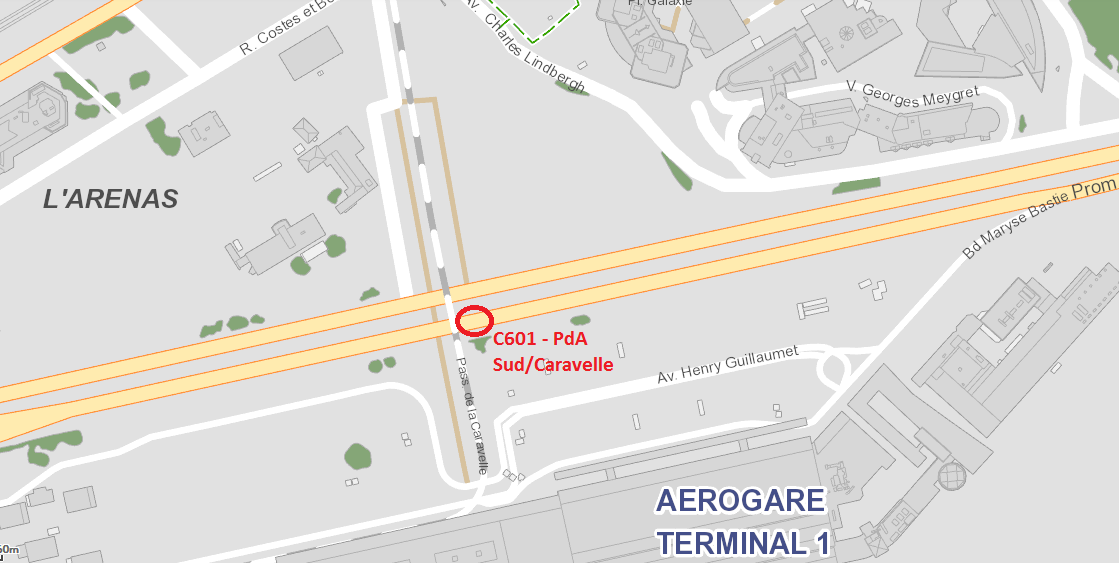
\includegraphics[scale=0.5]{terminal1.png}
    \caption{Location of C601 detector, close to Nice airport (south lane)}
    \label{fig:3.1}
\end{figure}

\emph{\small Figure 3.1 Location of C601 detector, close to Nice airport (south lane)}

    \begin{figure}
    \centering
    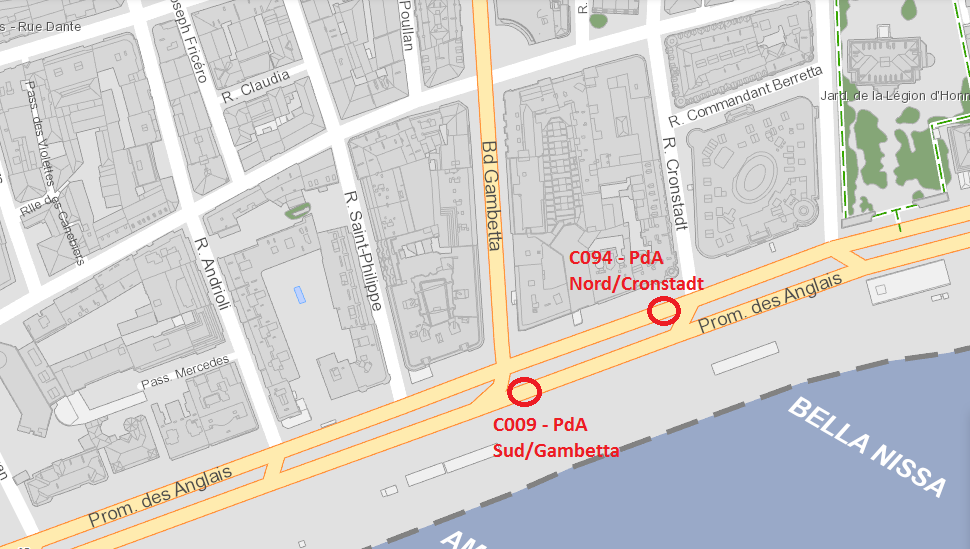
\includegraphics[scale=0.5]{gambetta cronstadt.png}
    \caption{Location of C009 and C094 detector, Nice city center (north and south lanes)}
    \label{fig:3.2}
\end{figure}

\emph{\small Figure 3.2 Location of C009 and C094 detector, Nice city center (north and south lanes)}

    \hypertarget{c601}{%
\subsubsection{C601}\label{c601}}

    To have an idea of the dynamic of the traffic over the all periods
available, the simple moving average with a window size of one week is
computed for C601 detector located near the airport, terminal 1. As
showed in Figure (3.\ref{fig:3.3}), the traffic in term of \(q(t,x)\)
(number of veh/h) presents seasonal behaviours. I can distinguish three
different levels of traffic also detected by the Kernel K-means
algorithm in Figure (3.\ref{fig:3.4}). The most trafficated periods are
from the beginning of June until the second week of July and from the
beginning of September to the third week of October. The less
trafficated period is the summer that coincides roughly with the school
break: from 5/7 to 2/9. The winter period from the third week of October
to the third week of December (before Christmas Holidays) has a low
level of traffic compared with the September period.

    \begin{figure}
    \centering
    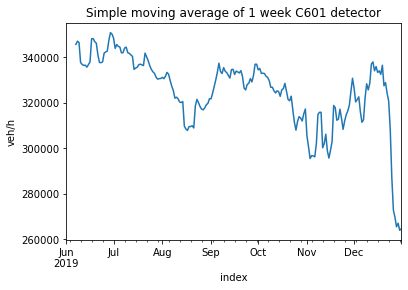
\includegraphics[scale=0.5]{SMA C601 2019.png}
    \caption{Detector C601: simple moving average 2019 period, flow (veh/h)}
    \label{fig:3.3}
\end{figure}

\emph{\small Figure 3.3 Detector C601: simple moving average 2019 period, flow (veh/h)}

    In Figure (3.\ref{fig:3.4}), the Global Alignment Kernel is seeded in
the Kernel K-Means algorithm with four clusters. 214 bi-variate (flow
and occupancy rate) daily time series are taken as input. The Algorithm
in addition to the three seasonal behaviours listed above recognizes
also the no-working days (Saturdays, Sundays and Public Holidays
\footnote{6/10/2019 Whit Monday, 15/08/2019 
Assumption of Mary, 11/11/2019 
Armistice Day}).

    \begin{figure}
    \centering
    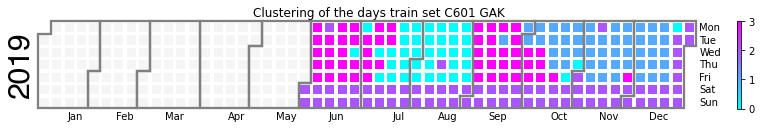
\includegraphics{GAK C601 2019 K=4.png}
    \caption{Detector C601: Kernel K-means, four clusters 2019 period}
    \label{fig:3.4}
\end{figure}

\emph{\small Figure 3.4 Detector C601: Kernel K-means, four clusters 2019 period}

    In Figure (3.\ref{fig:3.5}) a random sample of bi-variate time series
for each cluster is represented. To better render each cluster, after
all time series are assigned with Kernel K-Means, the centroids of the
clusters are computed using softDTW Equation (\(\ref{eq:12}\)). The
\(\gamma\) parameter is set to 42 using Equations (\(\ref{eq:7}\)) and
(\(\ref{eq:9}\)). The first cluster \(k=0\) identifies the summer in
which the peak of the morning is flatter than the ones present in the
second \(k=1\) and fourth \(k=3\) clusters for both flow and occupancy
rates. The second cluster \(k=1\) identifies the winter behaviour, where
the occupancy rate in the range 10:00 - 16:00 is lower than the ones
present in the fourth cluster \(k=3\). The third cluster \(k=2\)
portrays the dynamic of the traffic during no-working days, where during
the morning hours 7:00 - 10:00 the traffic level remains low. The fourth
cluster \(k=3\) describes the most trafficated period in which even
outside traffic peaks in the morning and in the afternoon the occupancy
rate registers higher values with respect to the other clusters.

    \begin{figure}
    \centering
    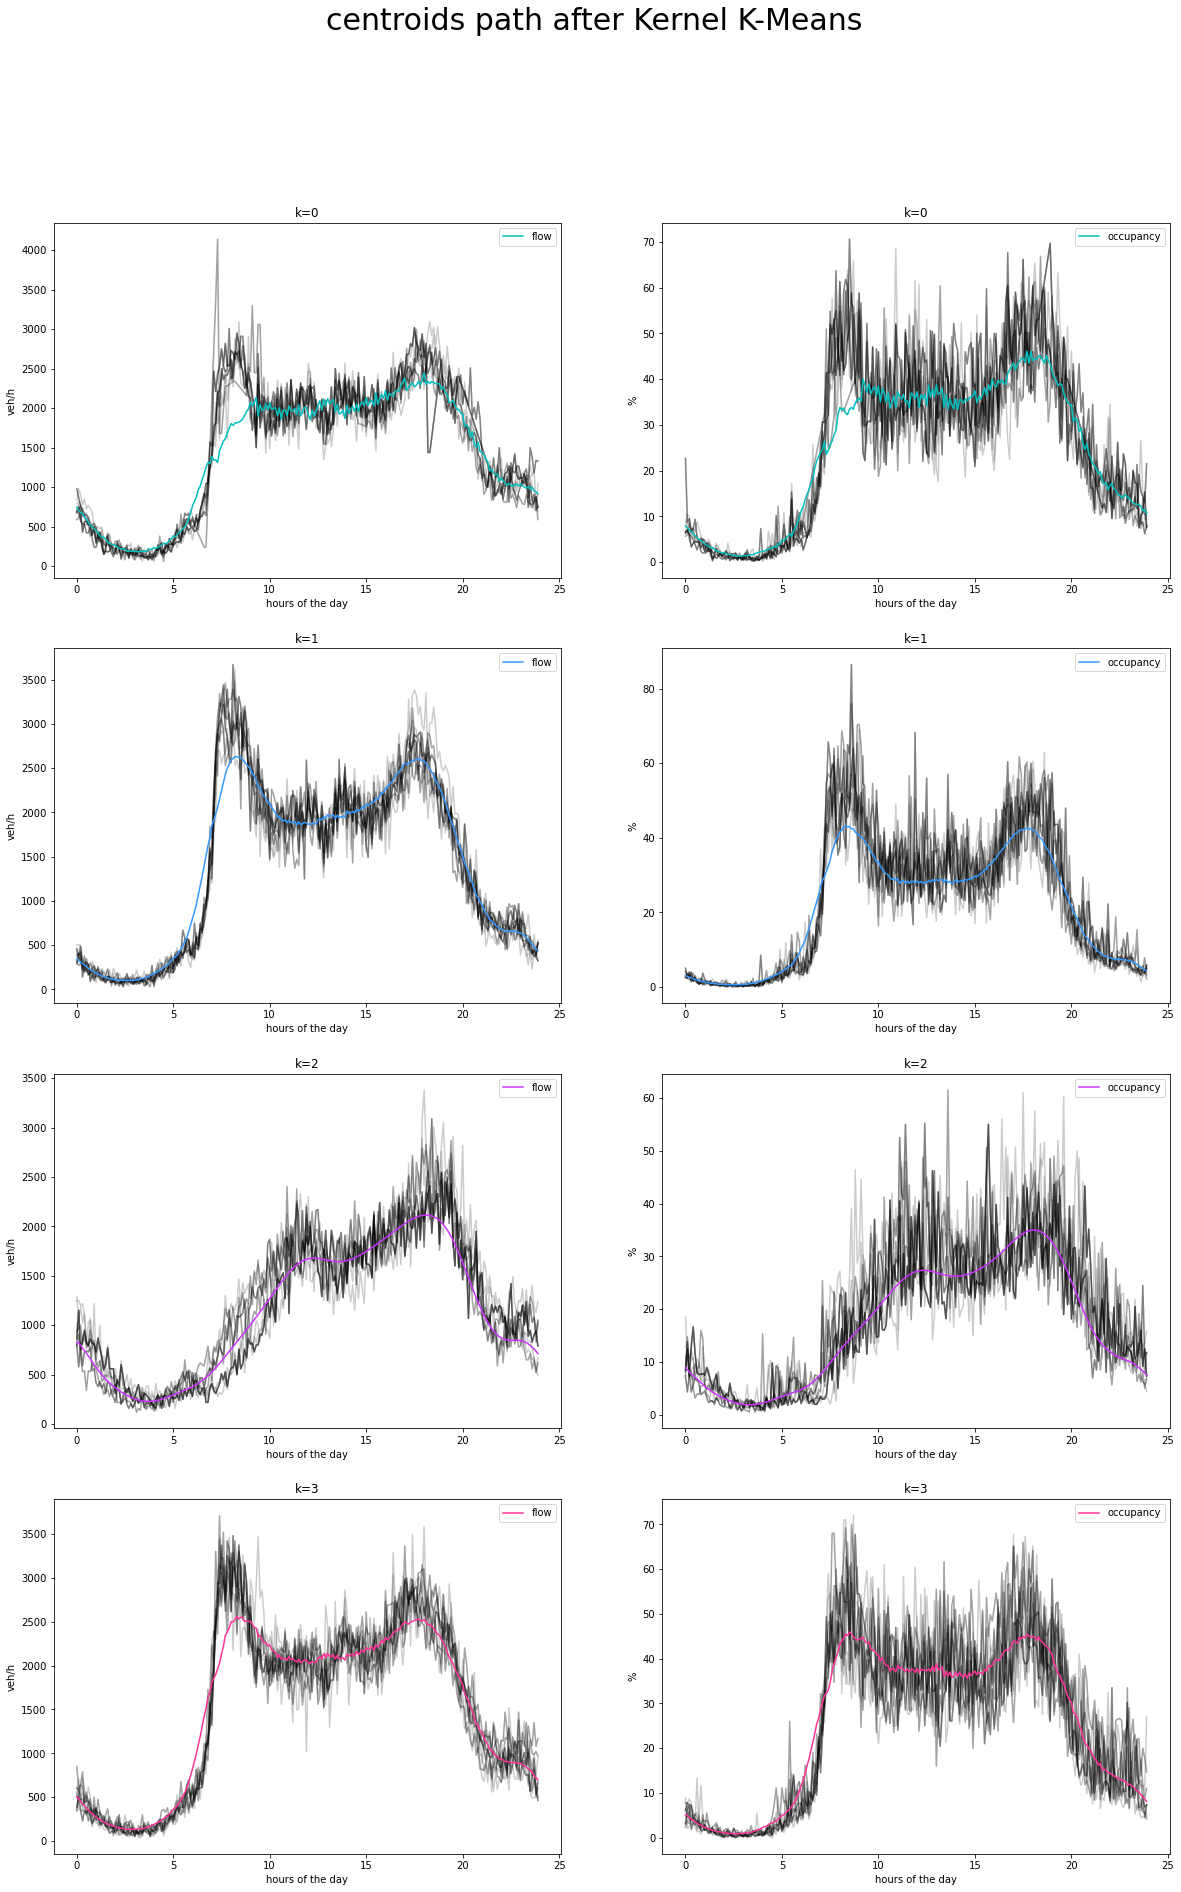
\includegraphics{GAK centroids K=4 2019.png}
    \caption{Detector C601: centroids of Kernel K-means, four clusters 2019 period, computed with softDTW}
    \label{fig:3.5}
\end{figure}

\emph{\small Figure 3.5 Detector C601: centroids of Kernel K-means, four clusters 2019 period, computed with softDTW}

    In Figure (3.\ref{fig:3.6}), to better distinguish the behaviour of the
first \(k=0\) and fourth \(k=3\) cluster weekly series of flow (veh/h)
of August and September are compared. The September serie presents a
higher level of traffic especially in the morninings.

    \begin{figure}
    \centering
    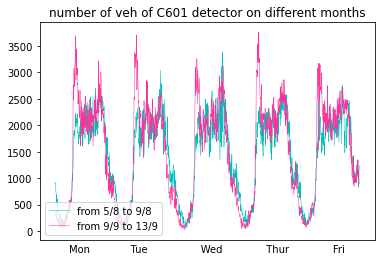
\includegraphics[scale=0.5]{GAK august vs september 2019.png}
    \caption{Detector C601: comparison of working days in a week of August and September 2019}
    \label{fig:3.6}
\end{figure}

\emph{\small Figure 3.6 Detector C601: comparison of working days in a week of August and September 2019 }

    In Figure (3.\ref{fig:3.7}), only the subperiod from 2/9 to 21/12 is
considered. The Global Alignment Kernel is seeded in the Kernel K-Means
algorithm with four clusters. 111 bi-variate (flow and occupancy rate)
daily time series are taken as input. Despite some weekend days form a
unique cluster, the seasonal behaviour is once again confirmed with a
separation between September and the winter period starting from the
third week of October. To separate better these two behaviours in Figure
(3.\ref{fig:3.8}) weekly series of occupancy rate (\(\%\)) of September
and November are compared. As already mentioned the occupancy rate in
the interval 10:00 - 16:00 is the main difference between the two
periods.

    \begin{figure}
    \centering
    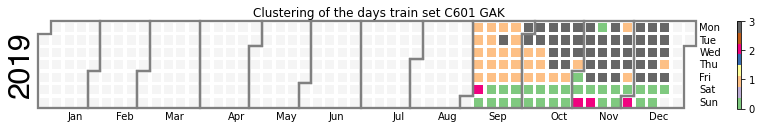
\includegraphics{GAK K=4 winter 2019.png}
    \caption{Detector C601: Kernel K-means, four cluster from 2/9/2019 to 21/12/2019}
    \label{fig:3.7}
\end{figure}

\emph{\small Figure 3.7 Detector C601: Kernel K-means, four cluster from 2/9/2019 to 21/12/2019}

    \begin{figure}
    \centering
    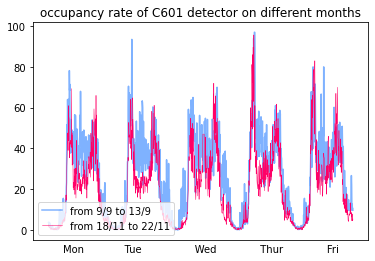
\includegraphics[scale=0.5]{C601 setember vs november 2019.png}
    \caption{Detector C601: comparison of working days in a week of September and November 2019}
    \label{fig:3.8}
\end{figure}

\emph{\small Figure 3.8 Detector C601: comparison of working days in a week of September and November 2019}

    \hypertarget{c009c094}{%
\subsubsection{C009/C094}\label{c009c094}}

    In this section results for C009/C094 are showed. C009 and C094 are used
in this section without any distinction, due to their proximity. The
algorithm and the moving average indicate a different behaviour of the
traffic especially in the summer months compared with the C601. This is
mainly due to the location of the detectors close to the city centre of
Nice and the beach as illustrated in Figure (3.\ref{fig:3.2}). In
particular, comparing Figure (3.\ref{fig:3.9}) with Figure
(3.\ref{fig:3.2})\$, the moving average of one week for C009 detctor
does not present an inflection in terms of flow (veh/h) in the two
centrals weeks.

    \begin{figure}
    \centering
    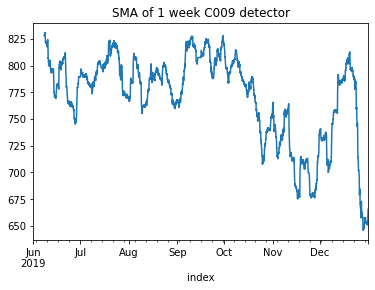
\includegraphics[scale=0.5]{SMA C009.png}
    \caption{}
    \label{fig:3.9}
\end{figure}

\emph{\small Figure 3.9 Detector C009: simple moving average 2019 period, flow (veh/h)}

    In Figure (3.\ref{fig:3.10}), the softDTW is seeded in the K-Means
algorithm with four clusters. The \(\gamma\) parameter estimated using
Equations (\(\ref{eq:7}\)) and (\(\ref{eq:9}\)) is set to 19. Again 214
bi-variate (flow and occupancy rate) daily time series are taken as
input. The Algorithm put together the month of August and Saturdays,
while Sundays form a separate. The remaining days of the week are
represent by the other two clusters, which mostly differ for the traffic
dynamic in the range 10:00 - 16:00 and in the range 20:00 - 24:00.

    \begin{figure}
    \centering
    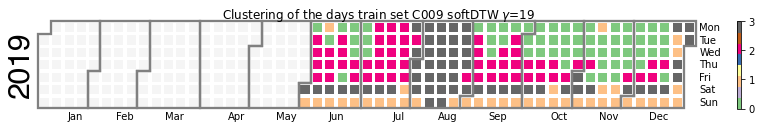
\includegraphics{softDTW C009 K=4 2019.png}
    \caption{Detector C009: K-means, four clusters 2019 period}
    \label{fig:3.10}
\end{figure}

\emph{\small Figure 3.10 Detector C009: K-means, four clusters 2019 period}

    In Figure (3.\ref{fig:3.11}), a random sample of bi-variate time series
for each cluster is represented with the corresponding centroid. The
first \(k=0\) and the third \(k=2\) cluster identify working days. I can
recognize the traffic peaks in the morning hours 7:30-9:30 and in the
afternoon hours 17:00-19:00. The second \(k=1\) and the fourth \(k=3\)
cluster represent the central part of the summer and no working days in
which the majority of the traffic is distributed in the central hours of
the day, without the morning peak. The level of traffic is more
consistent in the fourth cluster \(k=3\) than the second one \(k=1\),
with an higher level of flow and occupancy rate. In addition the level
of traffic remains significant until 20:00 in the fourth cluster \(k=3\)
while in the second one \(k=1\) starts to decrease before 20:00. The
first \(k=0\) and third \(k=2\) cluster mostly differ for the level of
traffic in the intervals 10:00-16:00 and 20:00-24:00. In these intervals
the third \(k=2\) cluster has higher values than the first one \(k=0\).
The third cluster \(k=2\) mostly maps the summer period June,July,
September (considered as months of work) and the last parts of working
days (Thursdays and Fridays) in October and December as showed in Figure
(3.\ref{fig:3.10}).

    \begin{figure}
    \centering
    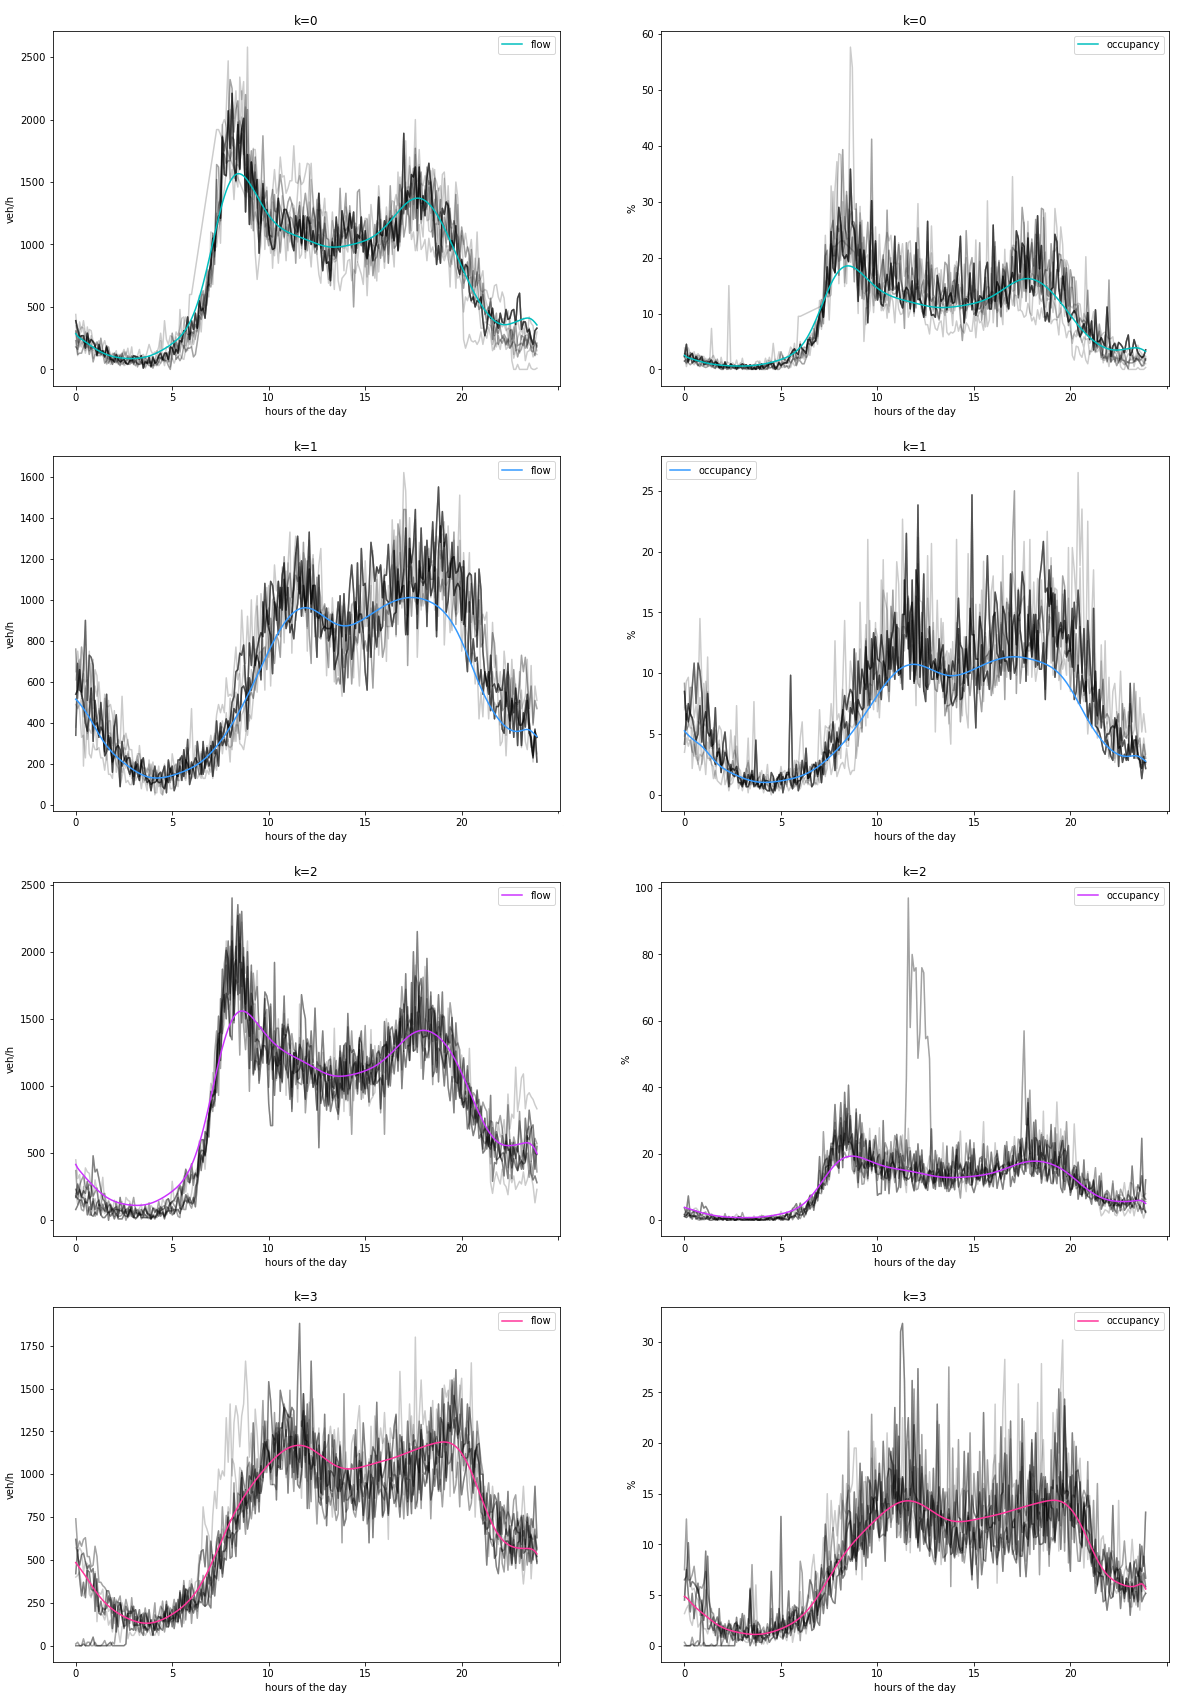
\includegraphics{softDTW centroids K=4 2019.png}
    \caption{Detector C009: centroids of K-means, four clusters 2019 period}
    \label{fig:3.11}
\end{figure}

\emph{\small Figure 3.11 Detector C009: centroids of K-means, four clusters 2019 period}

    To separate better the behaviours captured by the first \(k=0\) and
third \(k=2\) cluster in Figure (3.\ref{fig:3.12}) weekly series of the
flow of July and November are compared. I can see an higher level of
traffic in the evening in July series than in November series.

    \begin{figure}
    \centering
    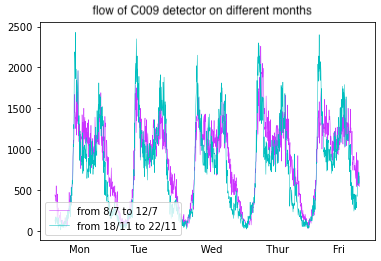
\includegraphics[scale=0.5]{softDTW july vs november 2019.png}
    \caption{Detector C009: comparison of working days in a week of July and November 2019}
    \label{fig:3.12}
\end{figure}

\emph{\small Figure 3.12 Detector C009: comparison of working days in a week of July and November 2019}

    In Figure (3.\ref{fig:3.13}) only the subperiod from 2/9 to 21/12 is
taken in account. The softDTW is seeded in the K-Means algorithm with
four clusters. The \(\gamma\) parameter estimated is set to 22. 111
bi-variate (flow and occupancy rate) daily time series are taken as
input. The Algorithm recognizes a day with aberrant data 5/12 in which
the detector was out of order for 6 hours. No working days form a unique
cluster,the fourth one \(k=3\), while working days are separated between
the first \(k=0\) and second \(k=1\) cluster. The second cluster \(k=1\)
maps mostly Thursdays and Fridays in the months of September, October
and December, while the first cluster \(k=0\) identifies the other
working days.

    \begin{figure}
    \centering
    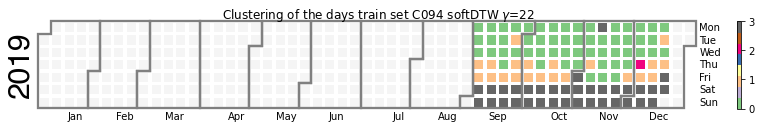
\includegraphics{softDTW K=4 winter 2019.png}
    \caption{Detector C094: K-means,four cluster from 2/9/2019 to 21/12/2019}
    \label{fig:3.13}
\end{figure}

\emph{\small Figure 3.13 Detector C094: K-means,four cluster from 2/9/2019 to 21/12/2019}

    In Figure (3.\ref{fig:3.14}) a random sample of bi-variate time series
for each cluster is represented with the corresponding centroid. The
second cluster \(k=1\) presents higher level of traffic than the first
one \(k=0\) in the morning 7:30-9:30, in the afternoon 17:00-19:00 and
in the evening 21:00-22:00. This tendency can be seen for both variables
flow and occupancy rate.

    \begin{figure}
    \centering
    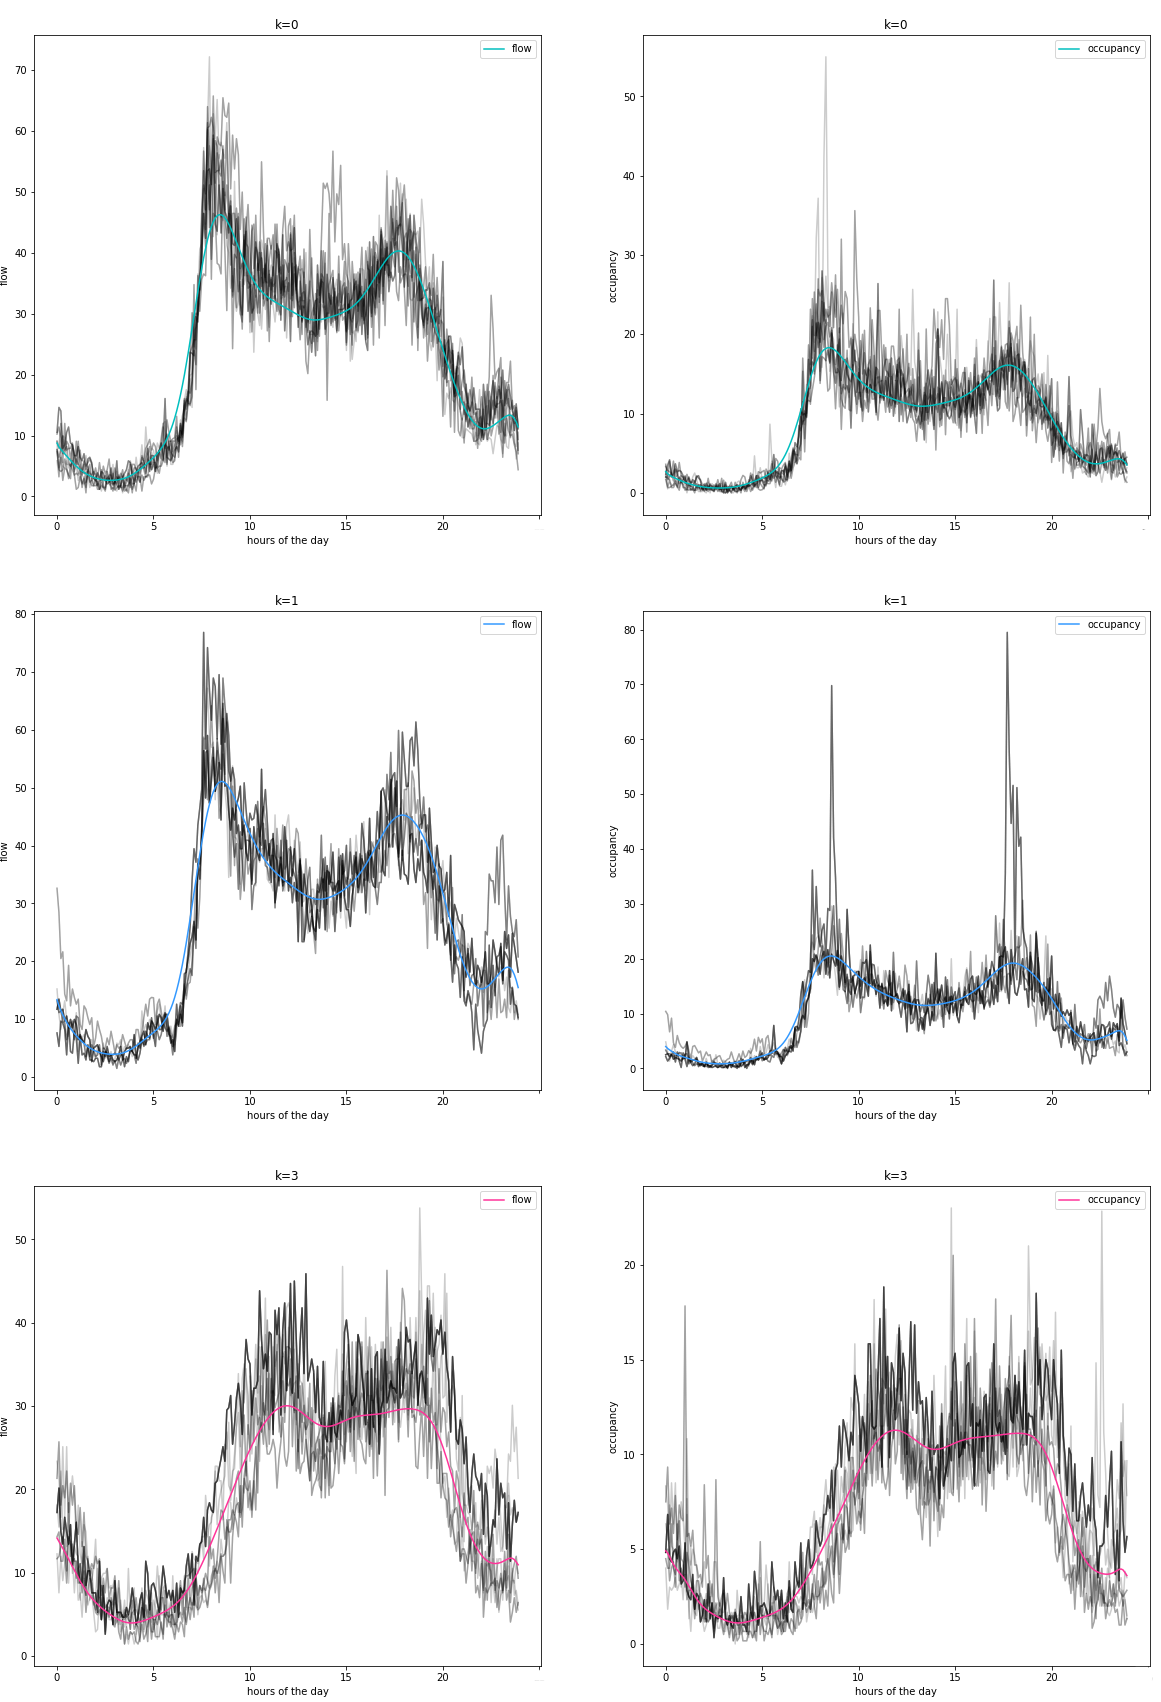
\includegraphics{softDTW centroids K=4 winter 2019.png}
    \caption{Detector C094: centroids of K-means, four clusters from 2/9/2019 to 21/12/2019}
    \label{fig:3.14}
\end{figure}

\emph{\small Figure 3.14 Detector C094: centroids of K-means, four clusters from 2/9/2019 to 21/12/2019}

    \subsection{2020}

    For the 2020 period all detectors were out of order from 11/11 to 24/11.
For this reason the effect of the second lockdown started 30/11 is not
competely studied. In addition, only 6 detectors are considered due to
other problems encountered in C077, C615 and C598 detectors, as
mentioned in the Appendix \ref{Appendix}. The locations of all detectors
are illustrated in Figure (3.\ref{fig:3.15}). Due to the impact of the
restrictions the clustering procedure give same result for each
detector. In this section results are showed with respect to detector
C601, but for all other detectors the classification of the days over
the 2020 period is the same.

    \begin{figure}
    \centering
    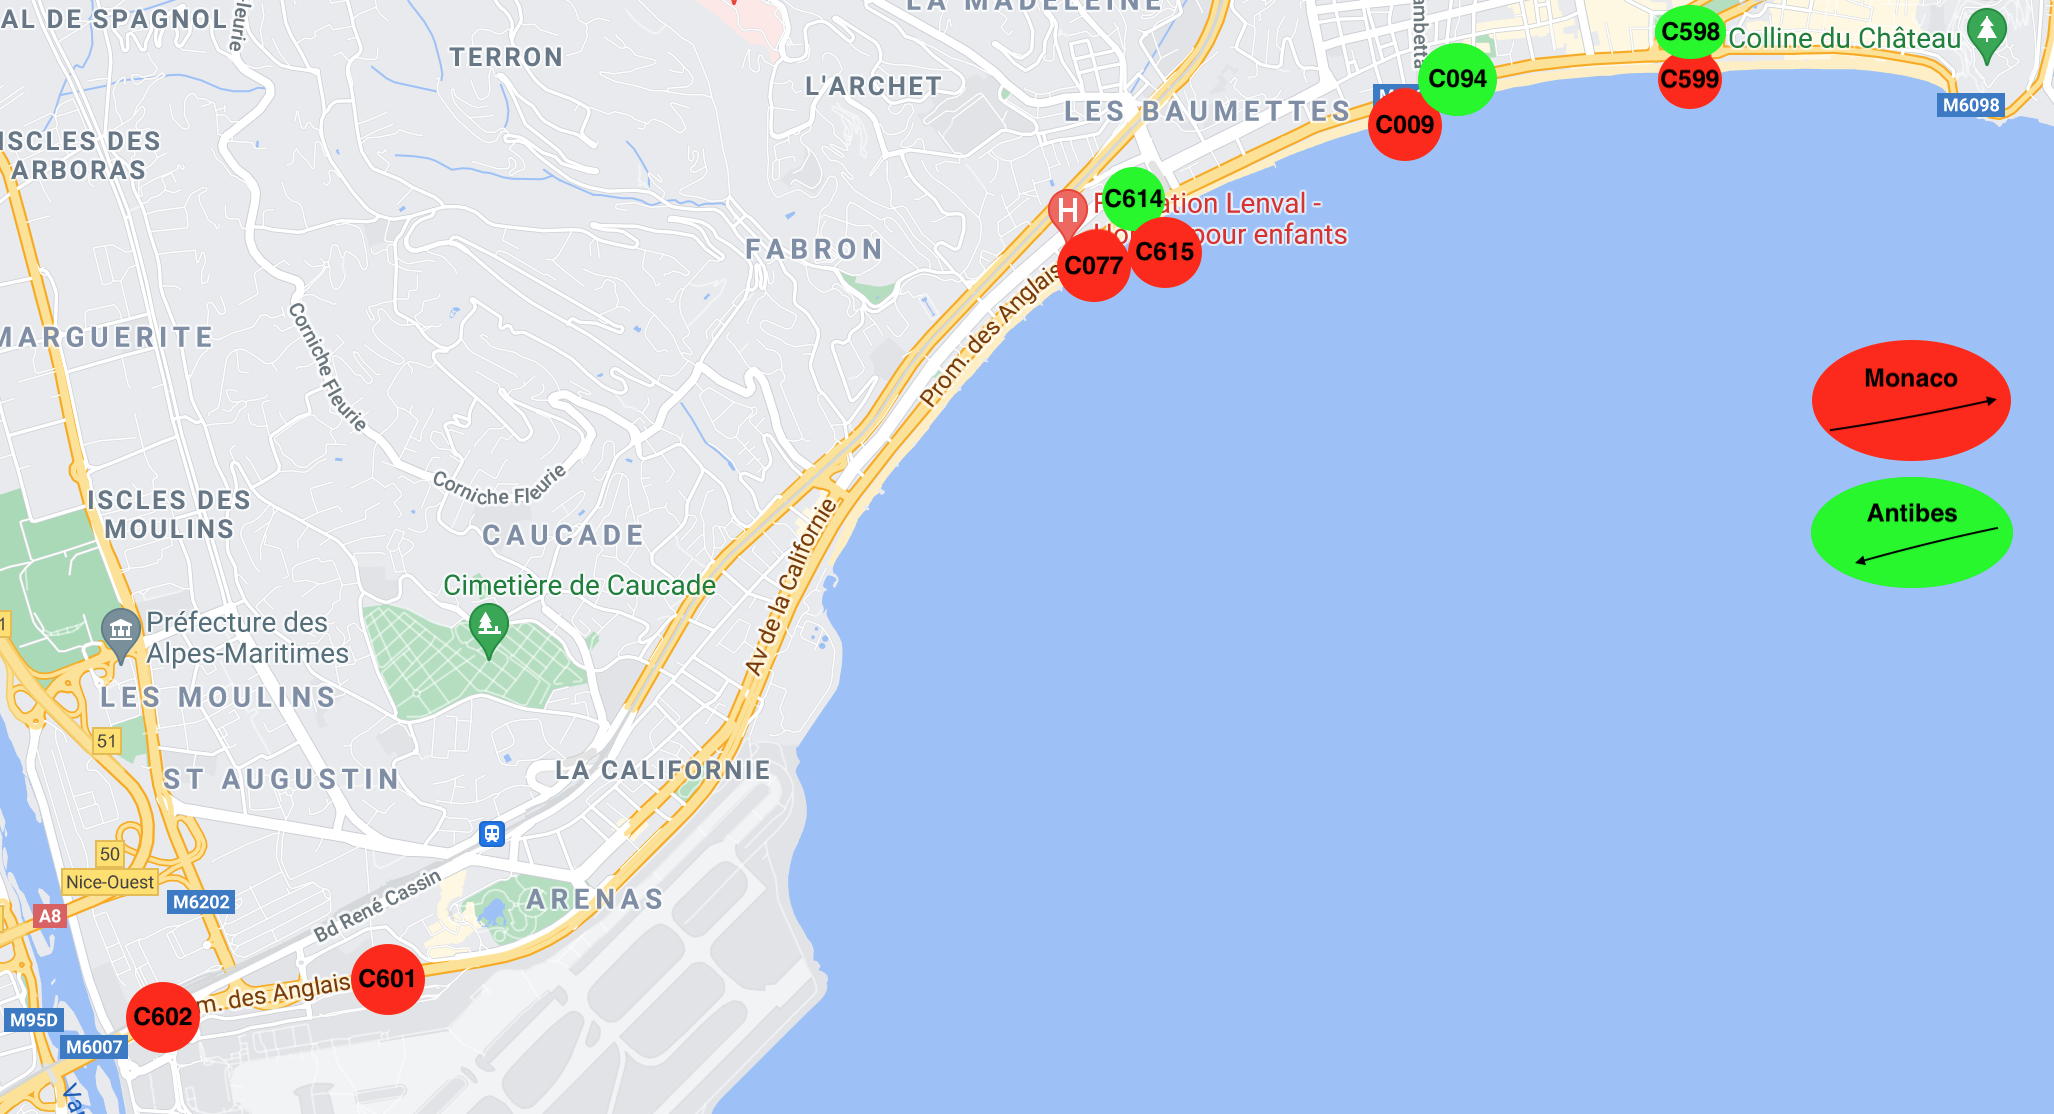
\includegraphics{detector promenade.png}
    \caption{Location of detectors Promenade Des Anglais}
    \label{fig:3.15}
\end{figure}

\emph{\small Figure 3.15 Location of detectors Promenade Des Anglais}

    The period considered for the analysis is from 6/2/2020 to 8/11/2020.
The simple moving average with a window size of one week is computed for
C601 detectors located near the airport, Terminal 1. As showed in Figure
(3.\ref{fig:3.16}), the traffic in term of \(q(t,x)\) (number of veh/h)
presents seasonal behaviours. I can clearly see the impact of the first
lockdown started the 17/03 and part of the second one started the 30/10.
The results showed below are from C601 detector, but repeating the
experiment with the data of the other detectors available I obtained the
same general tendency.

    \begin{figure}
    \centering
    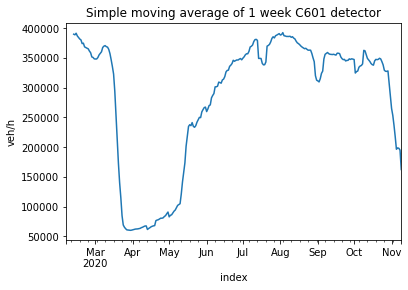
\includegraphics[scale=0.5]{SMA C601 2020.png}
    \caption{Detector C601: simple moving average 2020 period}
    \label{fig:3.16}
\end{figure}

\emph{\small Figure 3.16 Detector C601: simple moving average 2020 period}

    In Figure (3.\ref{fig:3.17}), the softDTW is seeded in K-Means algorithm
with five clusters. The \(\gamma\) parameter estimated is set to 29. 277
bi-variate (flow and occupancy rate) daily time series of detector C601
are taken as input. The algorithm distinguishes well the two phases of
the first lockdown detected by the third \(k=2\) and fourth \(k=3\)
cluster: from 17/03 to 11/05 ``stay home phase''(fourth cluster \(k=3\))
and from 11/05 to 02/06 where primary schools and some middle schools
were allowed to reopen (third cluster \(k=2\)). These two clusters
(\(k=2\) and \(k=3\)) identifies also the traffic behaviours in the
first days analyzed of the second lockdown from 30/10, where the fourth
\(k=3\) cluster maps no-working days and the third one \(k=2\)
identifies working days. The first cluster \(k=0\) represents working
days during the summer (from 6/7 to 29/8). The second cluster \(k=1\)
identifies no-working days in no-restriction period. The fifth cluster
\(k=4\) maps working days out of restriction periods and summer.

    \begin{figure}
    \centering
    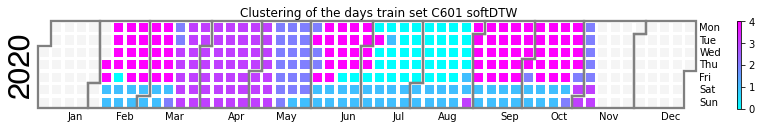
\includegraphics{softDTW K=5 2020.png}
    \caption{Detector C601:K-means, five clusters 2020 period}
    \label{fig:3.17}
\end{figure}

\emph{\small Figure 3.17 Detector C601:K-means, five clusters 2020 period}

    In Figure (3.\ref{fig:3.18}) a random sample of bi-variate time series
for each cluster is showed with the corresponding centroid. The fourth
cluster \(k=3\) (``stay home'' period) has the lowest level of traffic,
I can barely distinguish the traffic peak in the morning and in the
afternoon. The third cluster \(k=2\) (second part of first lockdown)
presents a higher level of traffic than the fourth one \(k=3\), with an
afternoon traffic peak greater than the one in the morning. The second
cluster \(k=1\) represents no-working days (Saturdays, Sundays and
public holidays) out of restriction periods, in which the highest level
of traffic is reached between 17:00-20:00 and the morning peak is
absent. The first cluster \(k=0\) and the fifth one \(k=4\) identifies
the most trafficated days. The fifth cluster \(k=4\) differ from the
first one \(k=0\) (July, August) for an higher peak of the traffic in
the morning hours (7:30-9:30).

    \begin{figure}
    \centering
    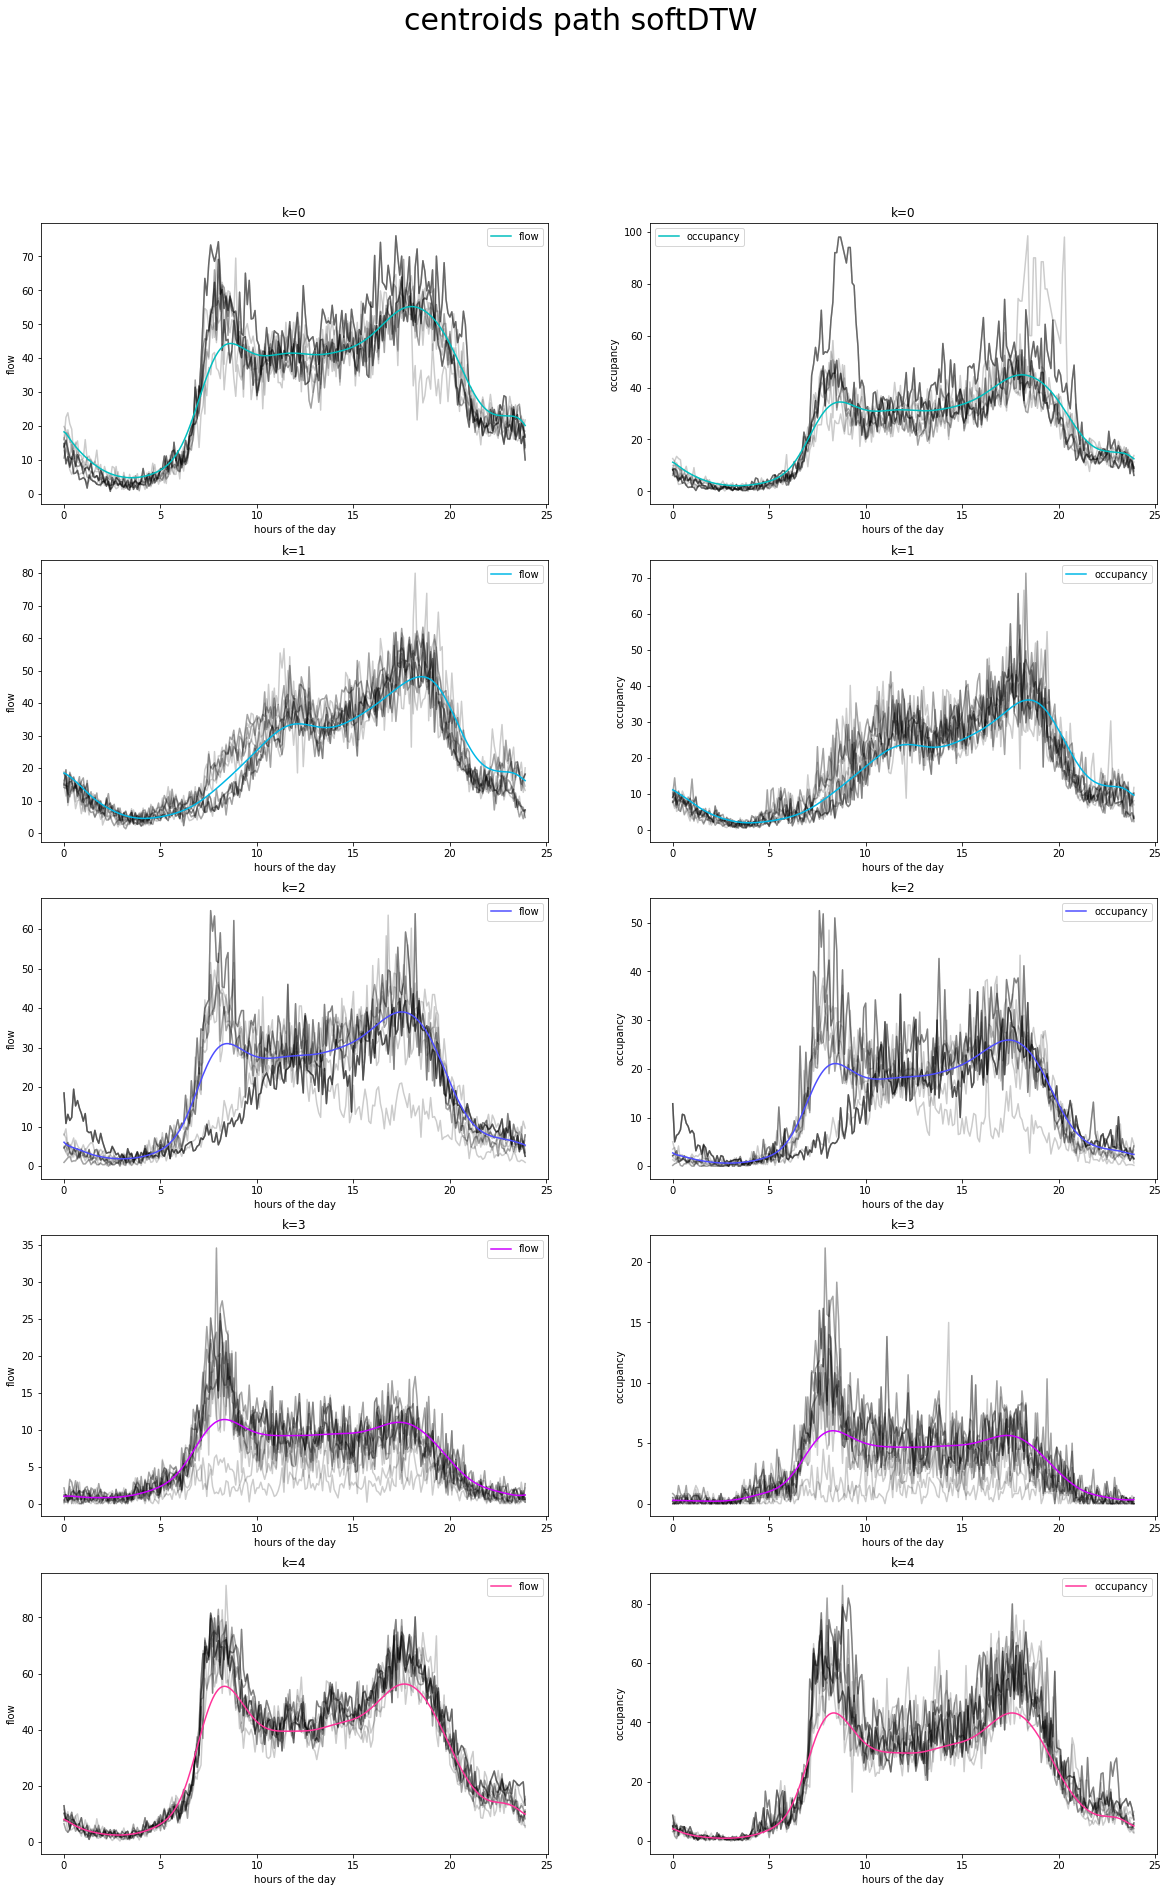
\includegraphics{softDTW centroids K=5 2020.png}
    \caption{Detector C601: centroids of K-means, five clusters 2020 period}
    \label{fig:3.18}
\end{figure}

\emph{\small Figure 3.18 Detector C601: centroids of K-means, five clusters 2020 period}

    In Figure (3.\ref{fig:3.19}), a comparison between a weekly flow series
of April and May is proposed to better visualize the discrepancy between
third \(k=2\) and fourth \(k=3\) cluster. The flow in the April series
(third cluster \(k=2\)) is really far from the level of flow in the May
series (fourth cluster \(k=3\)). The main impact of the restriction is
in the ``stay home'' period, while from 11/05 the traffic level
re-starts to grow.

    \begin{figure}
    \centering
    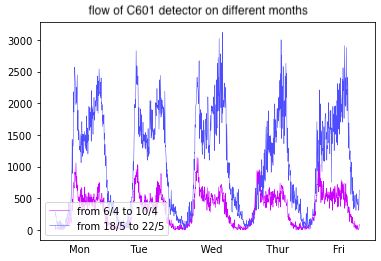
\includegraphics[scale=0.5]{C601 april vs may 2020.png}
    \caption{Detector C601: comparison of working days in a week of April and May 2020}
    \label{fig:3.19}
\end{figure}

\emph{\small Figure 3.19 Detector C601: comparison of working days in a week of April and May 2020}

    In Figure (3.\ref{fig:3.20}), a comparison between a weekly flow series
of August and September is showed to better visualize the difference
between the first \(k=0\) and fifth \(k=4\) cluster. The flow in
September series (fifth cluster \(k=5\)) presents peaks in the morning
hours higher than the ones in August series (first cluster \(k=0\)).

    \begin{figure}
    \centering
    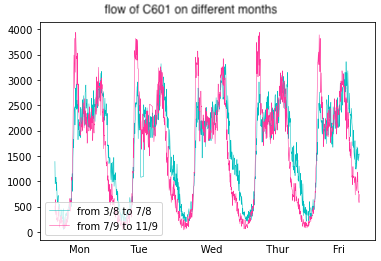
\includegraphics[scale=0.5]{C601 august vs september .png}
    \caption{Detector C601:comparison of working days in a week of August and September 2020}
    \label{fig:3.20}
\end{figure}

\emph{\small Figure 3.20 Detector C601:comparison of working days in a week of August and September 2020}

    \subsection{Comparison between 2020 and 2019}

    Plotting the flow against the occupancy rate for C094 detector for 2019
and 2020, I can see different layouts in the two years in Figure (3.21)
and Figure (3.22).\\
In Figure (3.21), representing 2019, data are more concentrated around
an occupancy rate of 20 \(\%\) and a flow of 1500 veh/h. In Figure
(3.22), representing instead the 2020, data are more scattered. Probably
in 2019 the traffic data are more concentrated in an area of the plot
than the one registered during 2020 due to the Covid restrictions
applied in 2020.

    \begin{figure}
\begin{tabular}{ll}
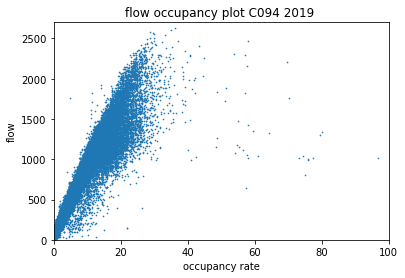
\includegraphics[scale=0.5]{FD C094 2019.png}
&
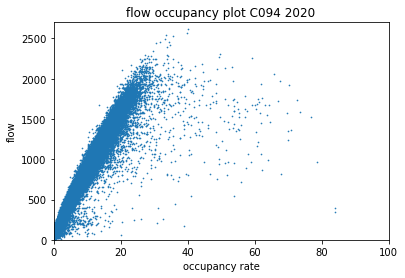
\includegraphics[scale=0.5]{FD C094 2020.png}
\end{tabular}
\caption{Left: 2019 
Right:2020}
\label{Fig:Race}
\end{figure}

\emph{\small Figure 3.21, 3.22 Detector C094: flow occupancy rate plot comparison}

    Despite different behaviour of traffic captured by fundamental diagrams
\cite{treiber2014traffic}(flow against occupancy plot), when considering
time series in specific periods of the years traffic dynamic seems very
similar. Restrictions applied during 2020 do not have a prolonged impact
of traffic dynamic. In fact by comparing the weekly flow series of the
second week of September for 2019 and 2020 the two series mostly
overlap, as showed in Figure (3.\ref{fig:3.23}).

    \begin{figure}
    \centering
    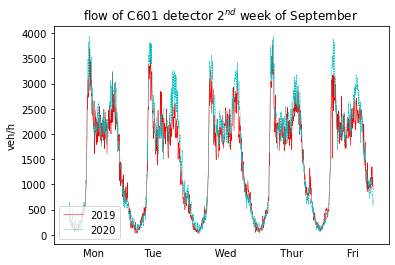
\includegraphics[scale=0.5]{september 2019 vs 2020 C601.png}
    \caption{Detector C601: comparison September 2020 and September 2019}
    \label{fig:3.23}
\end{figure}

\emph{\small Figure 3.23 Detector C601: comparison September 2020 and September 2019}

    In the flow serie of September 2020 the peaks in the morning and in the
afternoon seems to be slightly higher. Probably this reflects the higher
use of private cars with respect to public transport than in September
2019.

    \section{Voie Mathis}

    For ``Voie Mathis'' data are registered from 8 detectors: 4 detectors in
Monaco direction, the other ones in Antibes direction. The data used are
the speed \(v(t,x)\) (km/h) and the occupancy rate \(o(t,x)\) (\(\%\)).
They are registered every minute. The data are stored for the entire
year of 2019 while for 2020 no data are available from from 15/05 to
30/6 included. For this reason the impact of the first lockdown is not
studied. The location of the detectors is showed in Figure
(4.\ref{fig:4.1}) .

    \begin{figure}
    \centering
    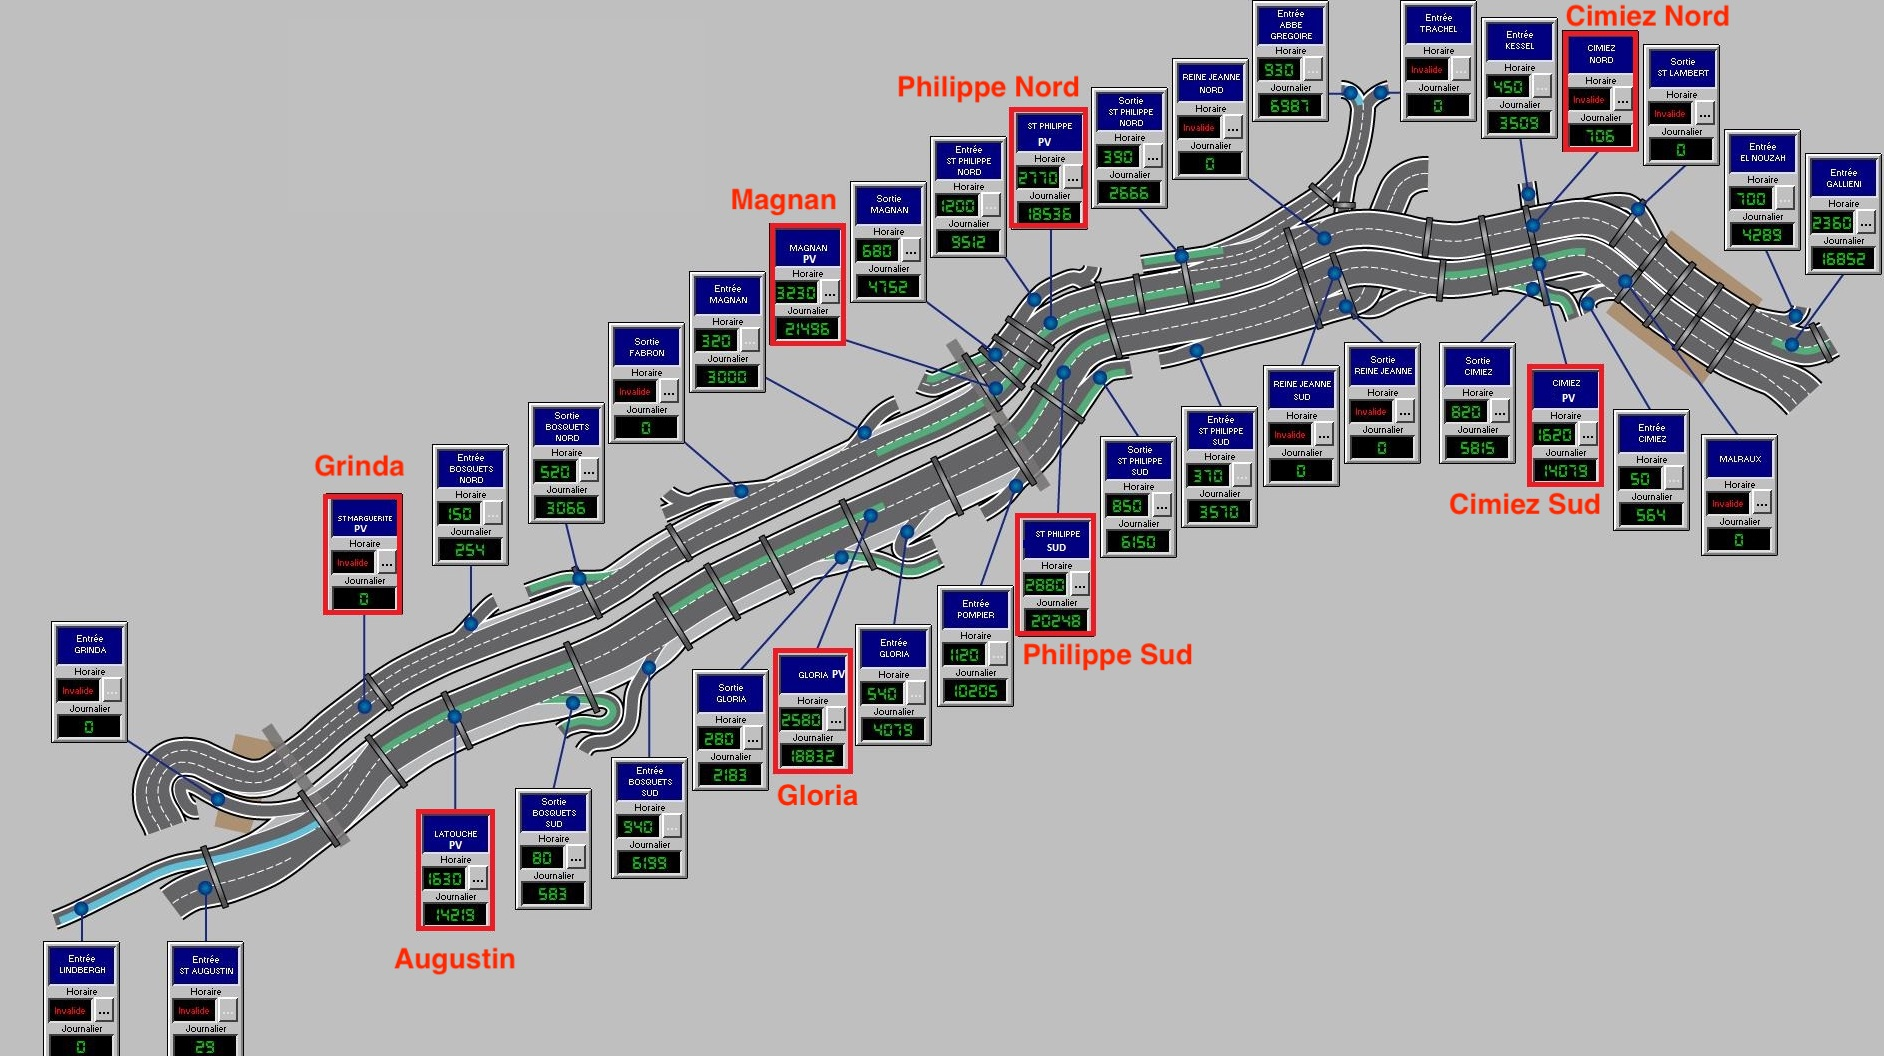
\includegraphics{detector voie mathis.JPG}
    \caption{Location of detectors on "Voie Mathis"}
    \label{fig:4.1}
\end{figure}

\emph{\small Figure 4.1 Location of detectors on "Voie Mathis"}

    Rough data need to be treated and aggregated. Here is a list of
operations computed in order to study the dynamics, in both intervals
time 2019 and 2020, for the occupancy rate and the speed:

\begin{enumerate}
\def\labelenumi{\arabic{enumi}.}
\item
  Extract for every lane of every detector the occupancy rate and the
  speed: 1-minute measurements.
\item
  Remove duplicates.
\item
  Fill missing values (jumps in the series).
\item
  Fill Nans with a preliminary imputation procedure: If an isolated Nan
  value is recognized (both previous and next observations are present),
  the observation before the Nan value is propagate forward to fill the
  missing value. This operation is computed only if the number of
  consecutive values is lower than 20 minutes (20 observation).
\item
  Mean of the lanes for every detector.
\item
  6-minute average.
\item
  Delete night observations from 00:00 to 5:00, due to the large
  quantities of Nans presents after the preliminary imputation procedure
  in the night hours.
\end{enumerate}

Despite this pre-process procedure some detectors present further
problems: a detailed list is presented in the Appendix
\(\ref{Appendix}\).

For ``Voie Mathis'' data the clustering procedure is applied with 2
different perspectives:

\begin{itemize}
\item
  (First perspective) all detectors univariate time series: the shape of
  time series is again \([ts,n,d]\), where \(d\) is the number of
  detectors considered. For this approach only the occupancy rate
  variable is taken in account for every detector due to the data
  available. In fact, as reported in Appendix \ref{Appendix} for
  Philippe sud detector speed measurements are not registered for both
  2019 and 2020.
\item
  (Second perspective) single detector multivariate time series: as with
  Promenade data the shape of the time series is \([ts,n,d]\), where
  \(d=2\) is the dimensionality of the daily multivariate time series
  (speed and occupancy rate).
\end{itemize}

For both perspectives the same normalization of Promenade data is used
over all periods (2019 and 2020). The choice of scaling \(d\) series
with respect to the entire periods and not with respect to the single
daily time series is done to preserve variability with respect to
different days of the week. As usual the inverse of the normalization
procedure is then applied in the centroids representations to have a
better comprehension of the paths.

    \subsection{comparison between first and second perspective}

    For 2019 data a comparison between first and second perspective is done
considering 3 clusters. For the first perspective, I considered 6
detectors occupancy rate time series of 365 days as input of K-means
seeded with softDTW. The resulting classification is showed in Figure
(4.\ref{fig:4.2}). The \(\gamma\) parameter is set to 11 using Equation
(\(\ref{eq:7}\)) and Equation ( \(\ref{eq:9}\)). The first cluster
\(k=0\) identifies no working days (Saturdays, Sundays,Public Holidays
\footnote{22/4 Easter Monday, 1/5 Labour day, 8/5 Victory in Europe Day, 30/5- 31/5 
Ascension Day, 10/6 Whit Monday, 14/7 Bastille Day, 1/11 All Saints' Day, 11/11 Armistice Day}
and the month of August). The second cluster \(k=1\) represents
``normal'' working days. The third cluster \(k=2\) maps working days in
periods in which there are school holidays
\footnote{Winter break from 9/2 to 25/9, Easter break from 6/4 to 23/4, Summer break from 5/7 to 2/9, All Saints' break from 19/10 to 4/11}
and majority of Wednesdays especially in the period September -
December.

    \begin{figure}
    \centering
    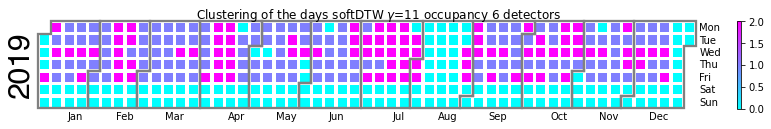
\includegraphics{softDTW K=3 2019.png}
    \caption{ K-means, three clusters 2019}
    \label{fig:4.2}
\end{figure}

\emph{\small Figure 4.2 K-means, three clusters 2019}

    In Figure (4.\ref{fig:4.3}) a random sample of time series for every
detector is represented with the corresponding centroid of the clusters.
For all detectors I can recognize the same tendency that distinguishes
the three clusters: the first cluster \(k=0\) does not present morning
and afternoon peaks, the second cluster \(k=1\) represents most
trafficated days while the third one \(k=2\) identifies working days
without ``school effect'' with morning and afternoon peaks lower than
the ones in the second cluster \(k=2\). As expected the level of traffic
between detectors is not the same, Cimiez Nord and Cimiez Sud detectors
seem to have in general a lower level of traffic than the other ones.

    \begin{figure}
    \centering
    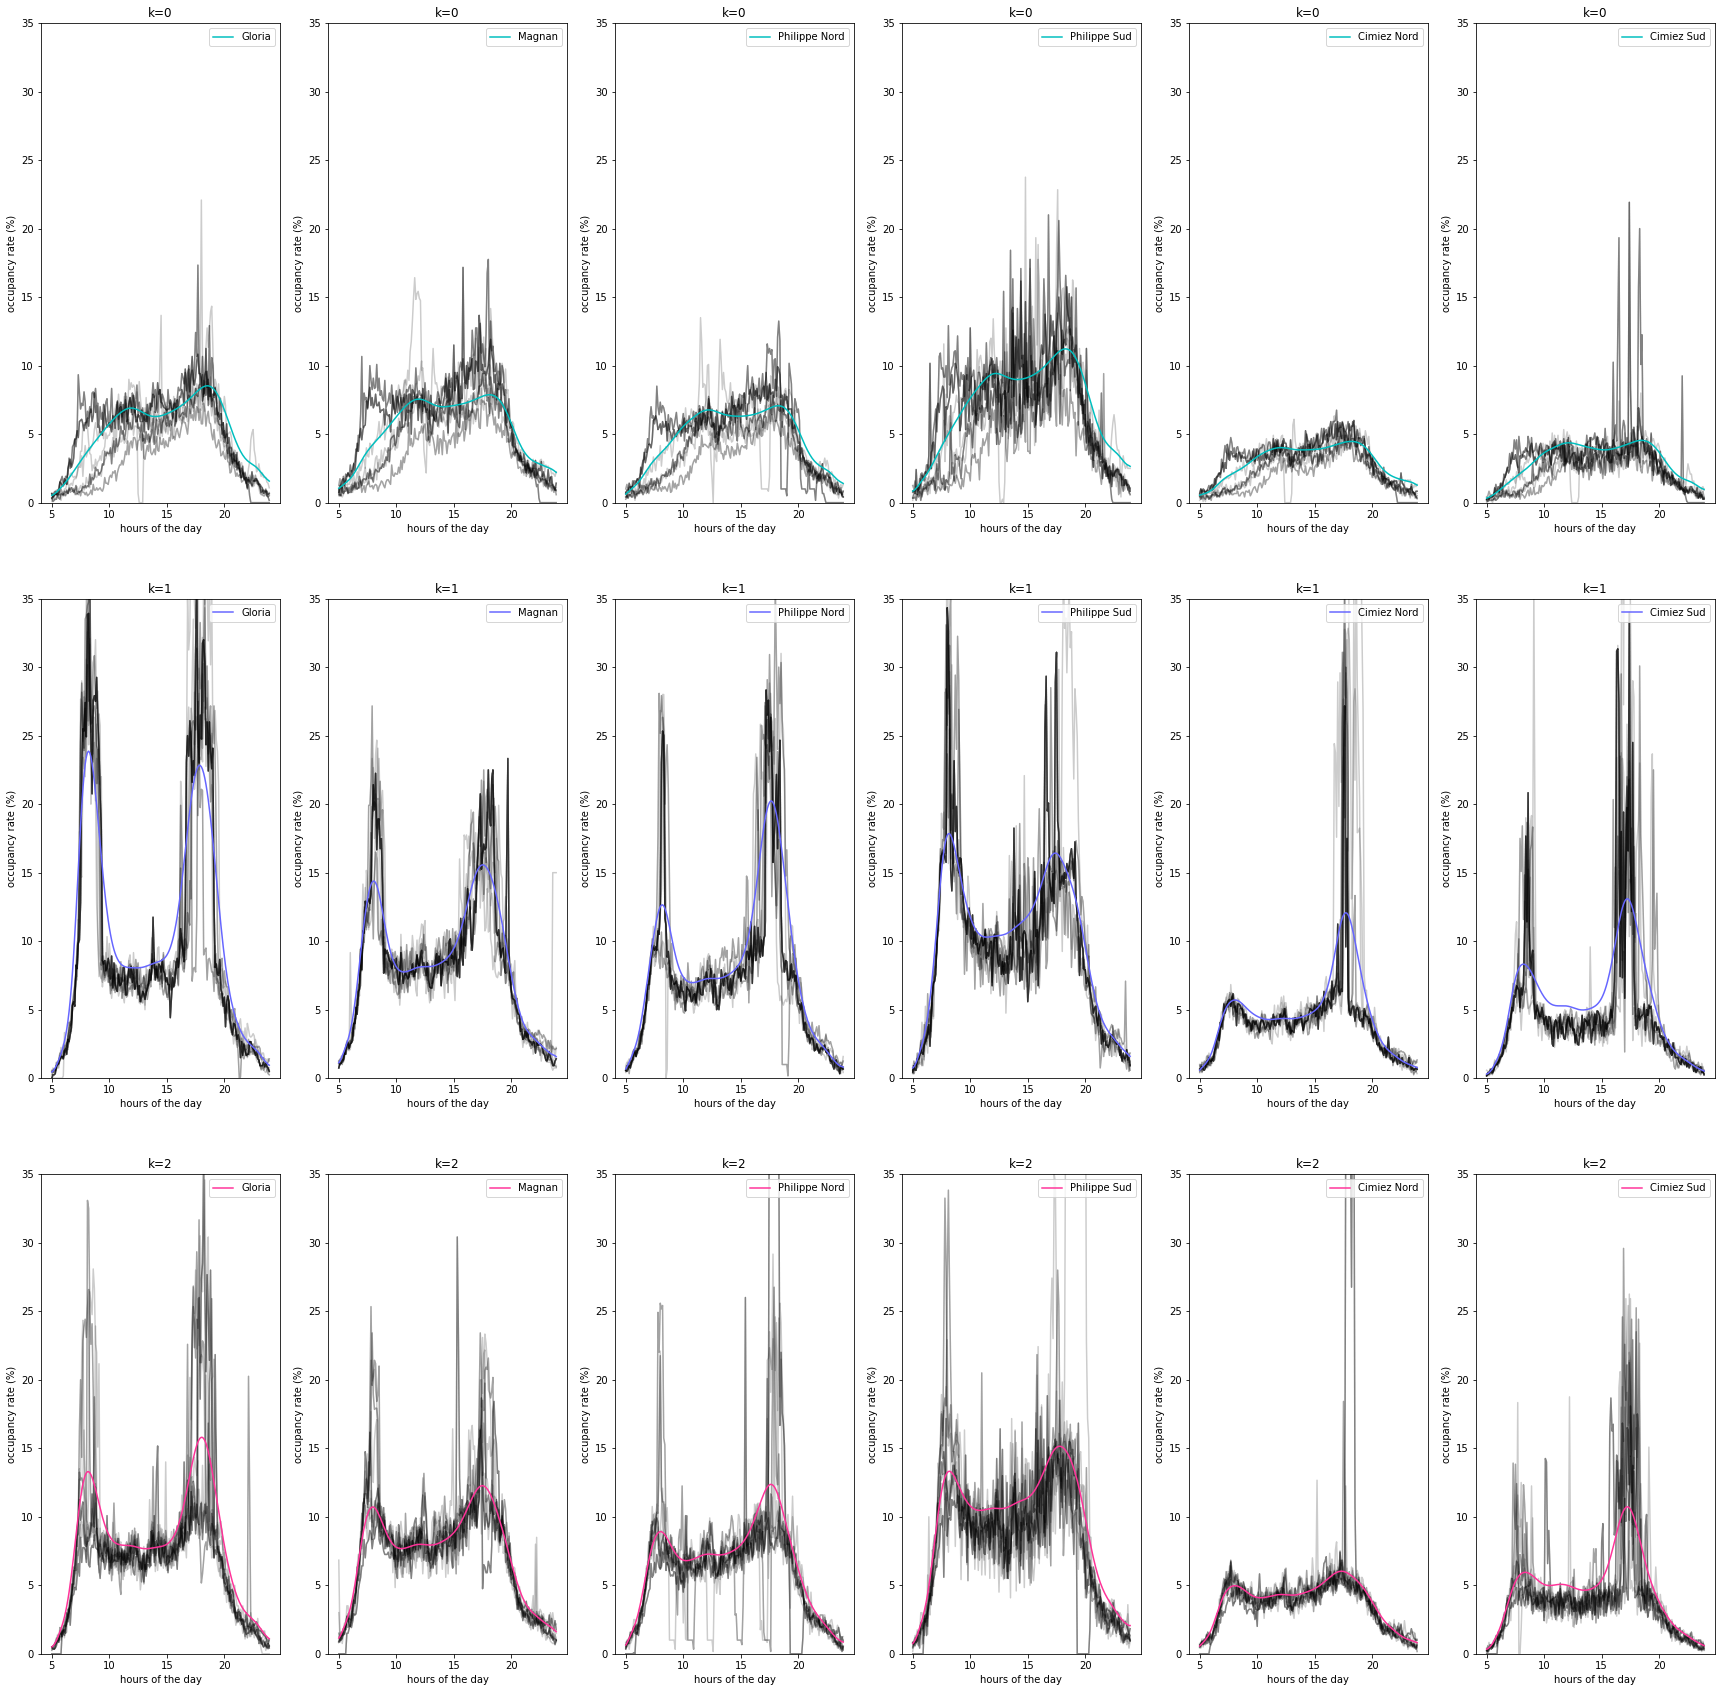
\includegraphics{centroids softDTW K=3 2019.png}
    \caption{centroids of K-means, three clusters 2019}
    \label{fig:4.3}
\end{figure}

\emph{\small Figure 4.3  centroids of K-means, three clusters 2019}

    For the second perspective, I considered the Gloria detector
multivariate time series (occupancy rate and speed) of 365 days as input
of K-means seeded with softDTW. The resulting classification is showed
in Figure (4.\ref{fig:4.4}). The \(\gamma\) parameter is set to 8 using
Equation (\(\ref{eq:7}\)) and Equation (\(\ref{eq:9}\)). The third
cluster \(k=2\), instead of capturing the traffic behaviour during
working days without ``school effect'' as in the first perspective
Figure (4.\ref{fig:4.2}), maps working days in the month of October,
November and December. The second cluster \(k=1\) represents the
remaining working days with the exception of the school holidays
\footnote{winter break from 9/2 to 25/9, the Easter break from 6/4 to 23/4 and Summer break from 5/7 to 2/9}
in which days are assigned to the first cluster \(k=0\) which maps no
working days.

    \begin{figure}
    \centering
    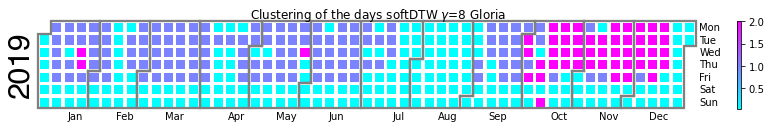
\includegraphics{softDTW K=3 gloria 2019.png}
    \caption{K-means, three clusters 2019 Gloria detector}
    \label{fig:4.4}
\end{figure}

\emph{\small Figure 4.4 K-means, three clusters 2019 Gloria detector}

    In Figure (4.\ref{fig:4.5}) a random sample of bi-variate time series
(speed and occupancy rate) for each cluster is showed with the
corresponding centroid. The first cluster \(k=0\) identifies no-working
days, it presents a free flow speed situation where the speed
represented by the centroid is almost equal to the speed limit (70 km/h)
for all day. The second cluster \(k=1\) is the most trafficated one,
with greater levels of congestion in the intervals 7-9 , 17-19 than the
ones in the third cluster \(k=2\). This is showed with greater level of
occupancy rate and lower level of speed during these hours in the
centroid of the second cluster \(k=1\).

    \begin{figure}
    \centering
    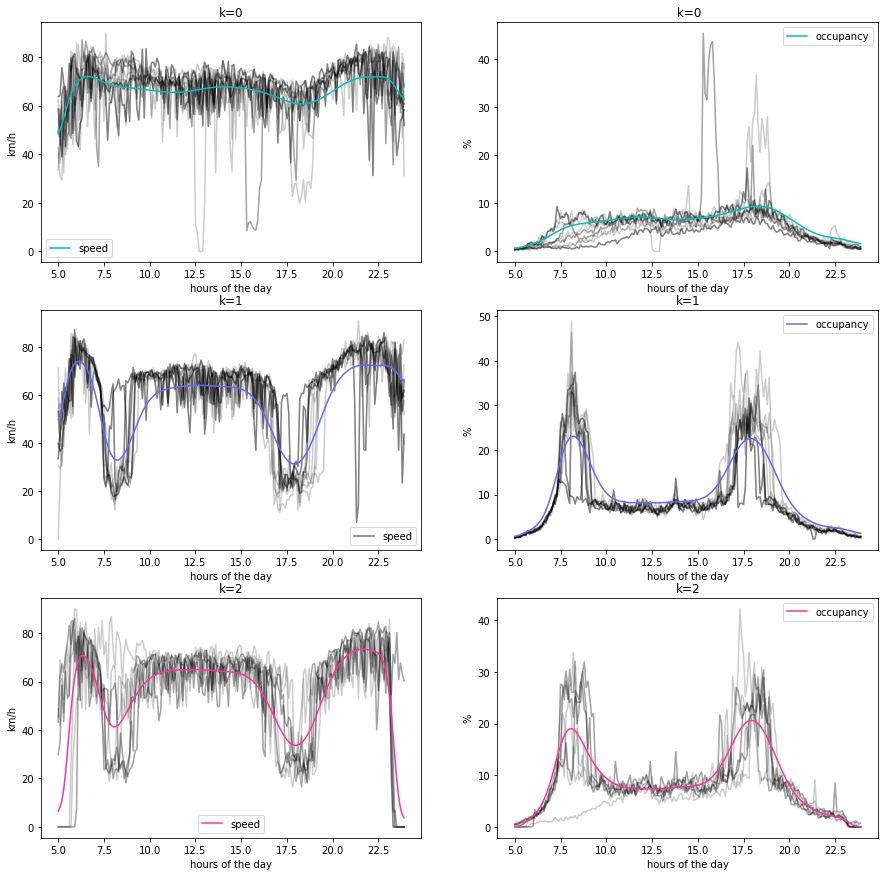
\includegraphics{centroids softDTW 2019 K=3 gloria.png}
    \caption{centroids of K-means, three clusters 2019 Gloria detector}
    \label{fig:4.5}
\end{figure}

\emph{\small Figure 4.5 centroids of K-means, three clusters 2019 Gloria detector}

    At a first glance, by using the first perspective, where all detectors
occupancy rate time series are taken into account, I can classify better
different traffic path of the days (Wednesday and ``school holidays'').
Probably by increasing the number of detectors (d \(\ggg\) 8) the task
of classify each working days in a cluster could be reached. However
``Voie Mathis'' traffic is caught only by 8 detectors. With the second
perspective instead, by looking at Gloria detector where the
multivariate time series of speed and occupancy rate is taken in
account, the algorithm captures mostly the seasonal behaviour where
working days in the months of October, November and December are
classified in the same cluster.

    \subsection{Train and Test validation of the first perspective}

    In this section the softDTW seeded with K-means algorithm is applied to
a set of data to train the centroids. Then the centroids are applied to
unseen data (test set). The train set are the occupancy rate time series
of 8 detectors from 2/9/2019 to 22/12/2019 while the test set are
occupancy rate time series of the same 8 detectors from 1/1/2020 to
3/1/2020. The choice of these train and test sets is done to use all the
8 detectors in a subperiods in which data are available for all of them
(see Appendix \ref{Appendix}). The number of cluster is set to 4, the
\(\gamma\) parameter is set to 22 using Equation (\(\ref{eq:7}\)) and
Equation (\(\ref{eq:9}\)). In Figure (4.\ref{fig:4.6}) the
classification of the days in the train set is showed. The first cluster
\(k=0\) identifies working days with a ``medium'' level of traffic
congestion. The second cluster \(k=1\) maps working days with a ``high''
level of traffic congestion especially during the afternoon peak. This
cluster \(k=1\) portrays half of the working days in the month of
November. The fourth cluster \(k=3\) represents working days with a
``low'' level of traffic congestion (days without ``school effect'').
The fourth cluster \(k=3\) mostly identifies Wednesdays and days during
All Saints' break (from 19/10 to 4/11).The third cluster \(k=2\) renders
no working days (Saturdays, Sundays and Public Holidays).

    \begin{figure}
    \centering
    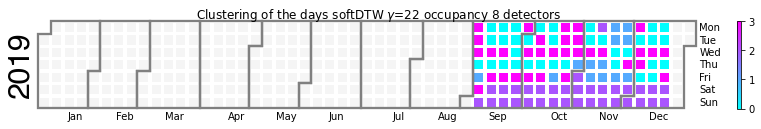
\includegraphics{softDTW K=4 sem2 2019 train.png}
    \caption{K-means, four clusters from 2/9/2019 to 22/12/2019: train set}
    \label{fig:4.6}
\end{figure}

\emph{\small Figure 4.6  K-means, four clusters from 2/9/2019 to 22/12/2019: train set}

    In Figure (4.\ref{fig:4.7}) a random sample of time series (train set)
for every detector is represented with the corresponding centroid of the
cluster. For all detectors I can recognize the same tendency that
distinguishes the four clusters. The first cluster \(k=0\) differ from
the second one \(k=1\) mostly for the peaks in the afternoon, where the
occupancy rate reached in the second cluster \(k=1\) tend to be higher
than the one reached in the first one \(k=0\). For Grinda detector also
the peak in the morning in the second cluster \(k=1\) is higher than the
one registered in the first cluster \(k=0\). The fourth cluster \(k=3\)
is the closest to the first cluster \(k=0\) but with a lower level of
traffic due to the absence of the ``school effect''. For 2 detectors
(Cimiez Nord and Grinda) I can barely distinguish the peaks in the
morning and in the afternoon. The third cluster \(k=2\) identifies no
working days in which the level of traffic remains quite from 11:00 to
19:00, without a defined morning peak.

    \begin{figure}
    \centering
    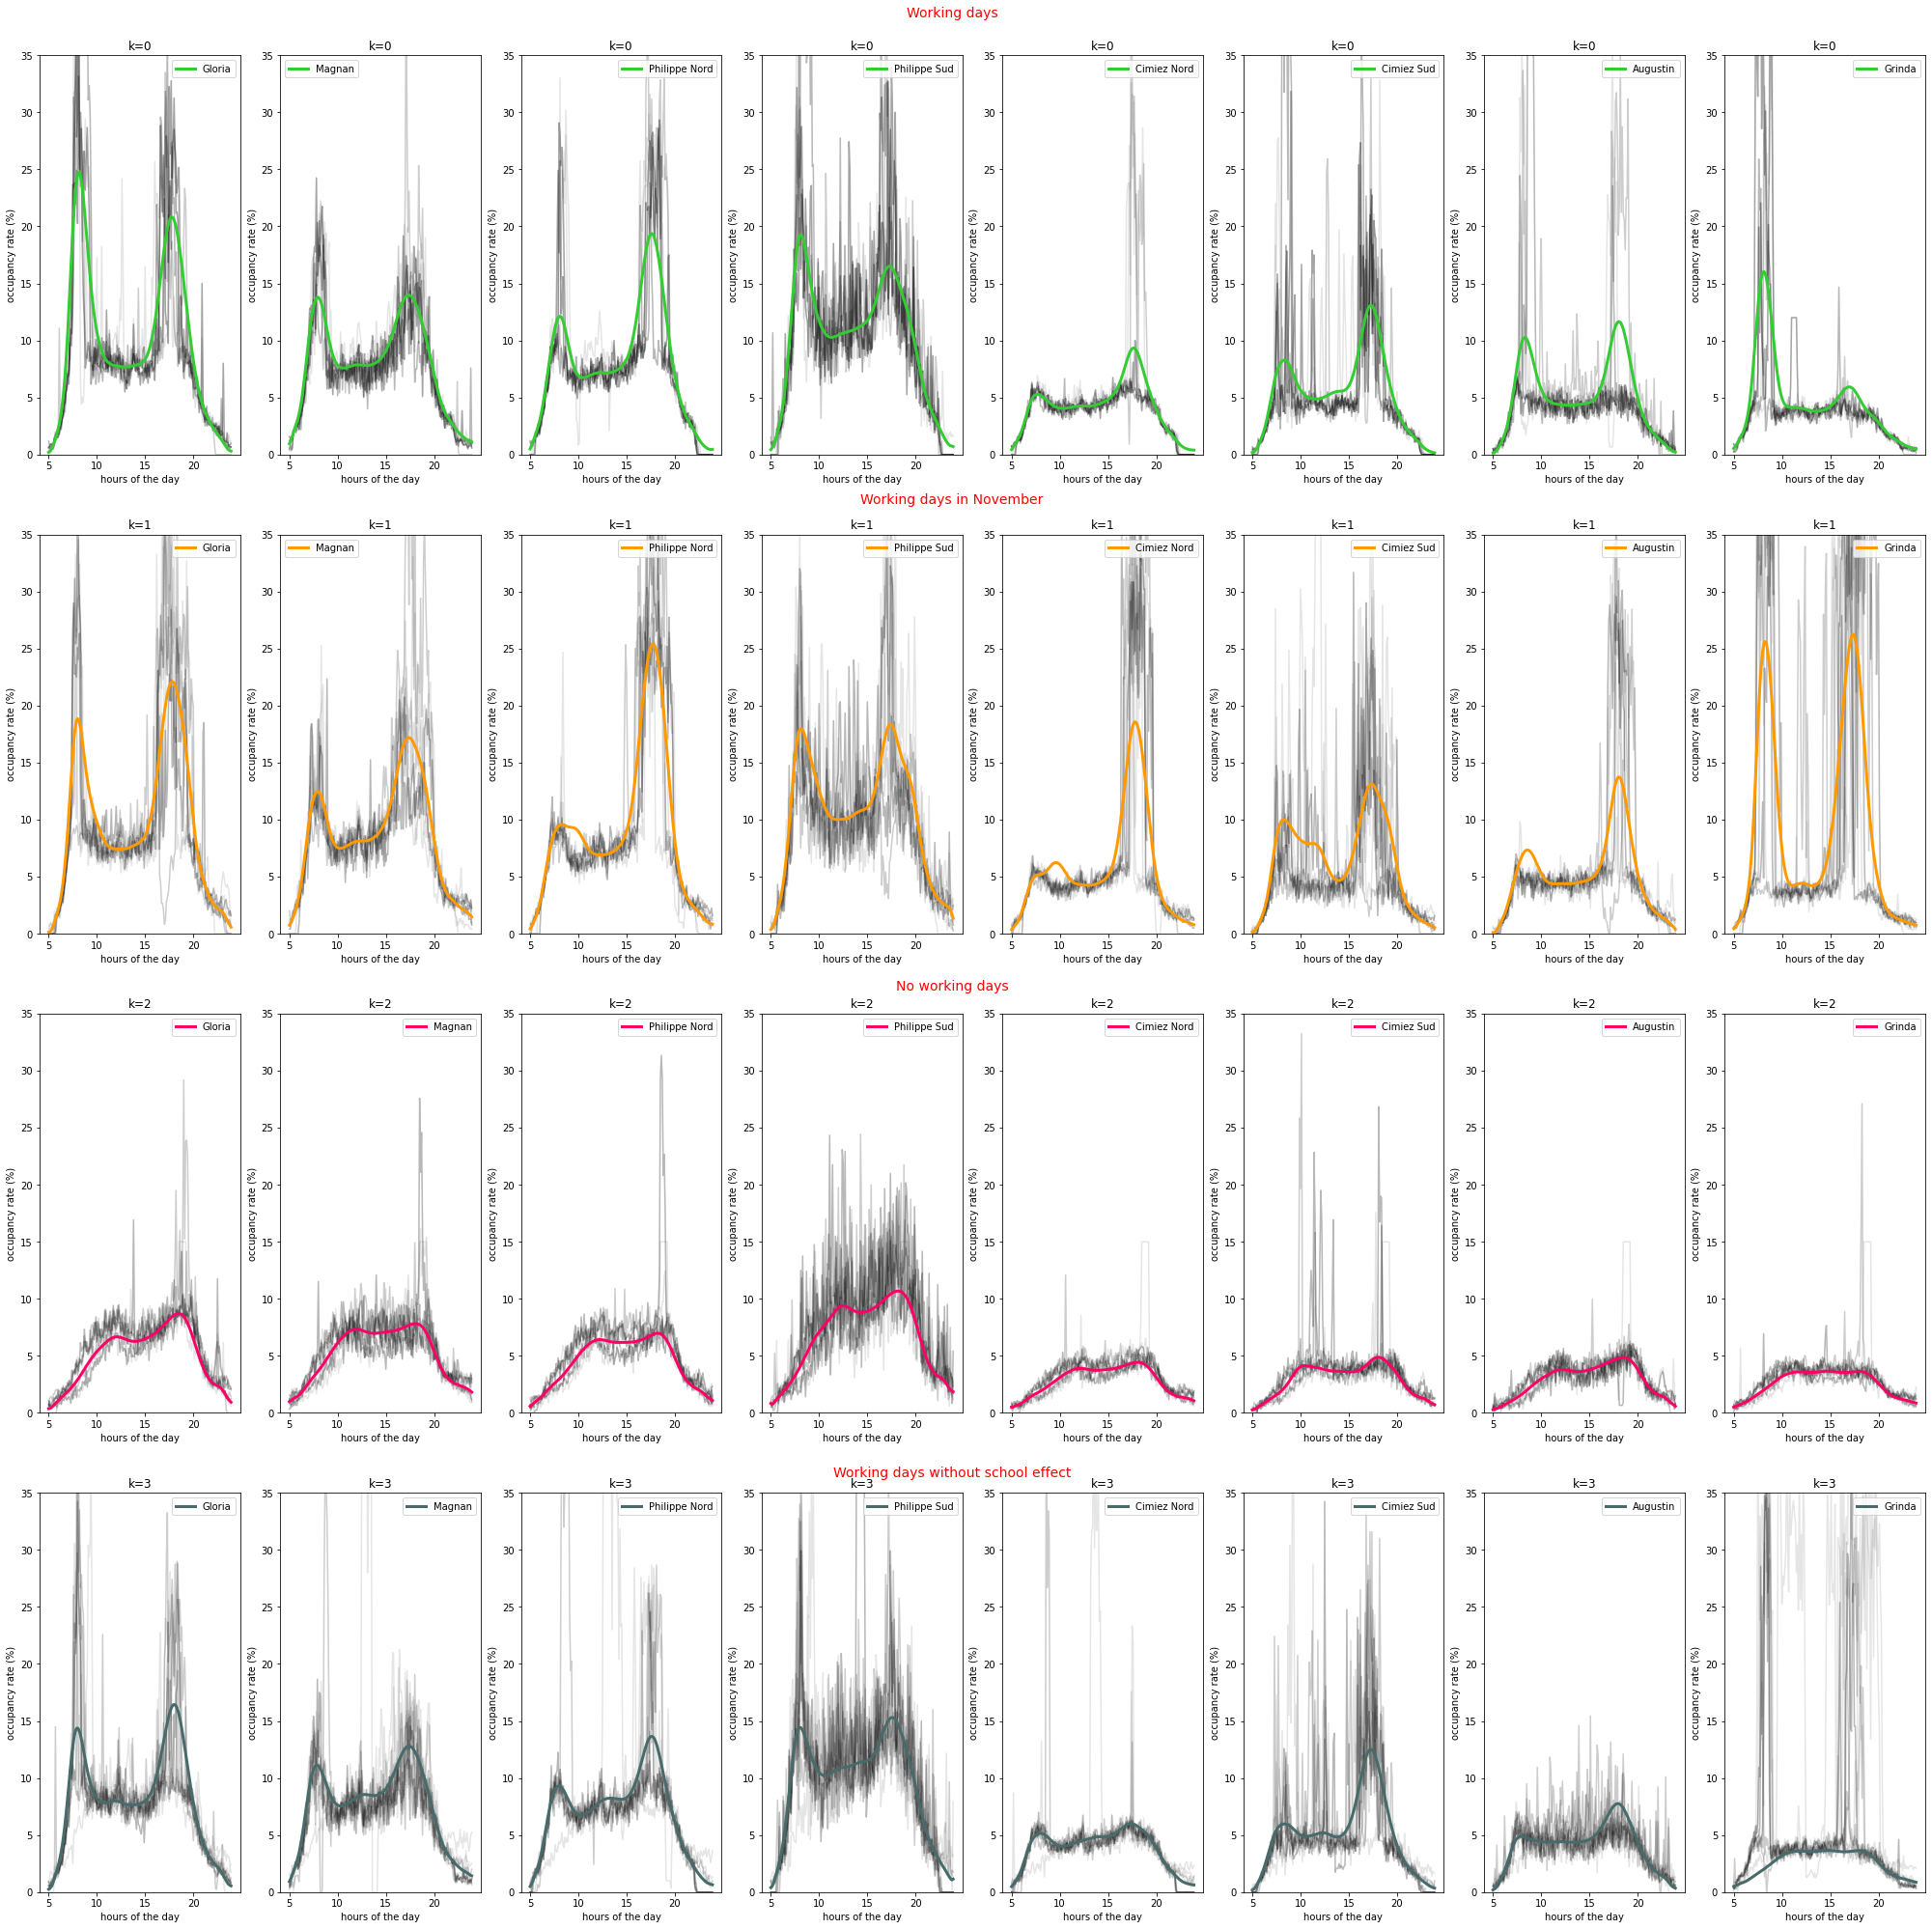
\includegraphics{centroids softDTW K=4 sem2 2019.png}
    \caption{centroids of K-means, four clusters from 2/9/2019 to 22/12/2019}
    \label{fig:4.7}
\end{figure}

\emph{\small Figure 4.7 centroids of K-means, four clusters from 2/9/2019 to 22/12/2019}

    In Figure (4.\ref{fig:4.8}) centroids showed above Figure
(4.\ref{fig:4.7}) are used to classify days in the test set. The third
cluster \(k=2\) continue to map no-working days including the last part
of Christmas holidays up to 6/1. The second cluster \(k=1\), the most
trafficated one, identifies only one day. The fourth cluster \(k=4\)
maps mostly Mondays, Wednesdays and days of winter school break
\footnote{ from 15/2 to 2/3 }, while the first cluster \(k=0\)
represents the other working days. These results confirm that the
traffic dynamic in the first months of 2020 is not equal to the dynamic
in the last months of 2019.

    \begin{figure}
    \centering
    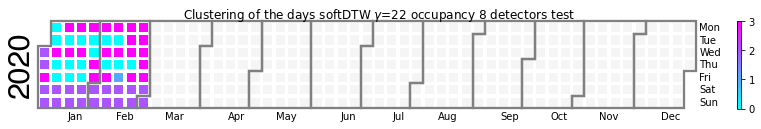
\includegraphics{softDTW K=4 2020 test.png}
    \caption{}
    \label{fig:4.8}
\end{figure}

\emph{\small Figure 4.8 K-means, four clusters from 1/1/2020 to 1/3/2020: test set}

    \subsection{2020 Impact of second lockdown with the first perspective}

    To analyze the impact of the restriction started the 30/10, I considered
6 detectors occupancy rate time series of the second semester 2020 as
input of K-means seeded with softDTW. The number of clusters is set to
2, the \(\gamma\) parameter is set to 6. In Figure (4.\ref{fig:4.9}) the
classification of the days is showed. The first cluster \(k=0\)
identifies no working-days \footnote{ Saturdays, Sundays, 13/7, 14/7 },
central weeks of August and the days of the second nationwide lockdown
from 30/10 to 1/12, in which non-essential businesses such as pubs and
restaurants were closed but schools and factories would remained open.
The second cluster \(k=1\) maps others working days. The impact of the
second lockdown is evident in the month of November, while starting from
the beginning of December the traffic re-starts to increase.

    \begin{figure}
    \centering
    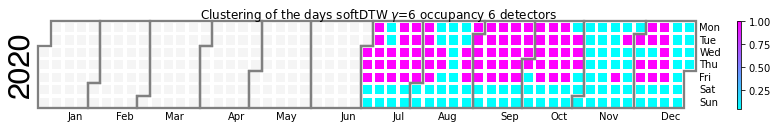
\includegraphics{softDTW K=2 sem2 2020.png}
    \caption{}
    \label{fig:4.9}
\end{figure}

\emph{\small Figure 4.9 K-means, two clusters from 31/8/2020 to 31/12/2020}

    In Figure 4.10 a random sample of time series (train set) for every
detector is represented with the corresponding centroid of the clusters.
The second cluster \(k=1\) mostly differ from the first one for the
level of traffic during the intervals 7:00-9:00 and 17:00-19:00. In the
second cluster \(k=1\) during these intervals the level of traffic
reaches the highest peaks. As expected these peaks are not visible in
the first cluster \(k=0\) representing no-working days, or days in which
non-essential businesses were closed due to restriction.

    \begin{figure}
    \centering
    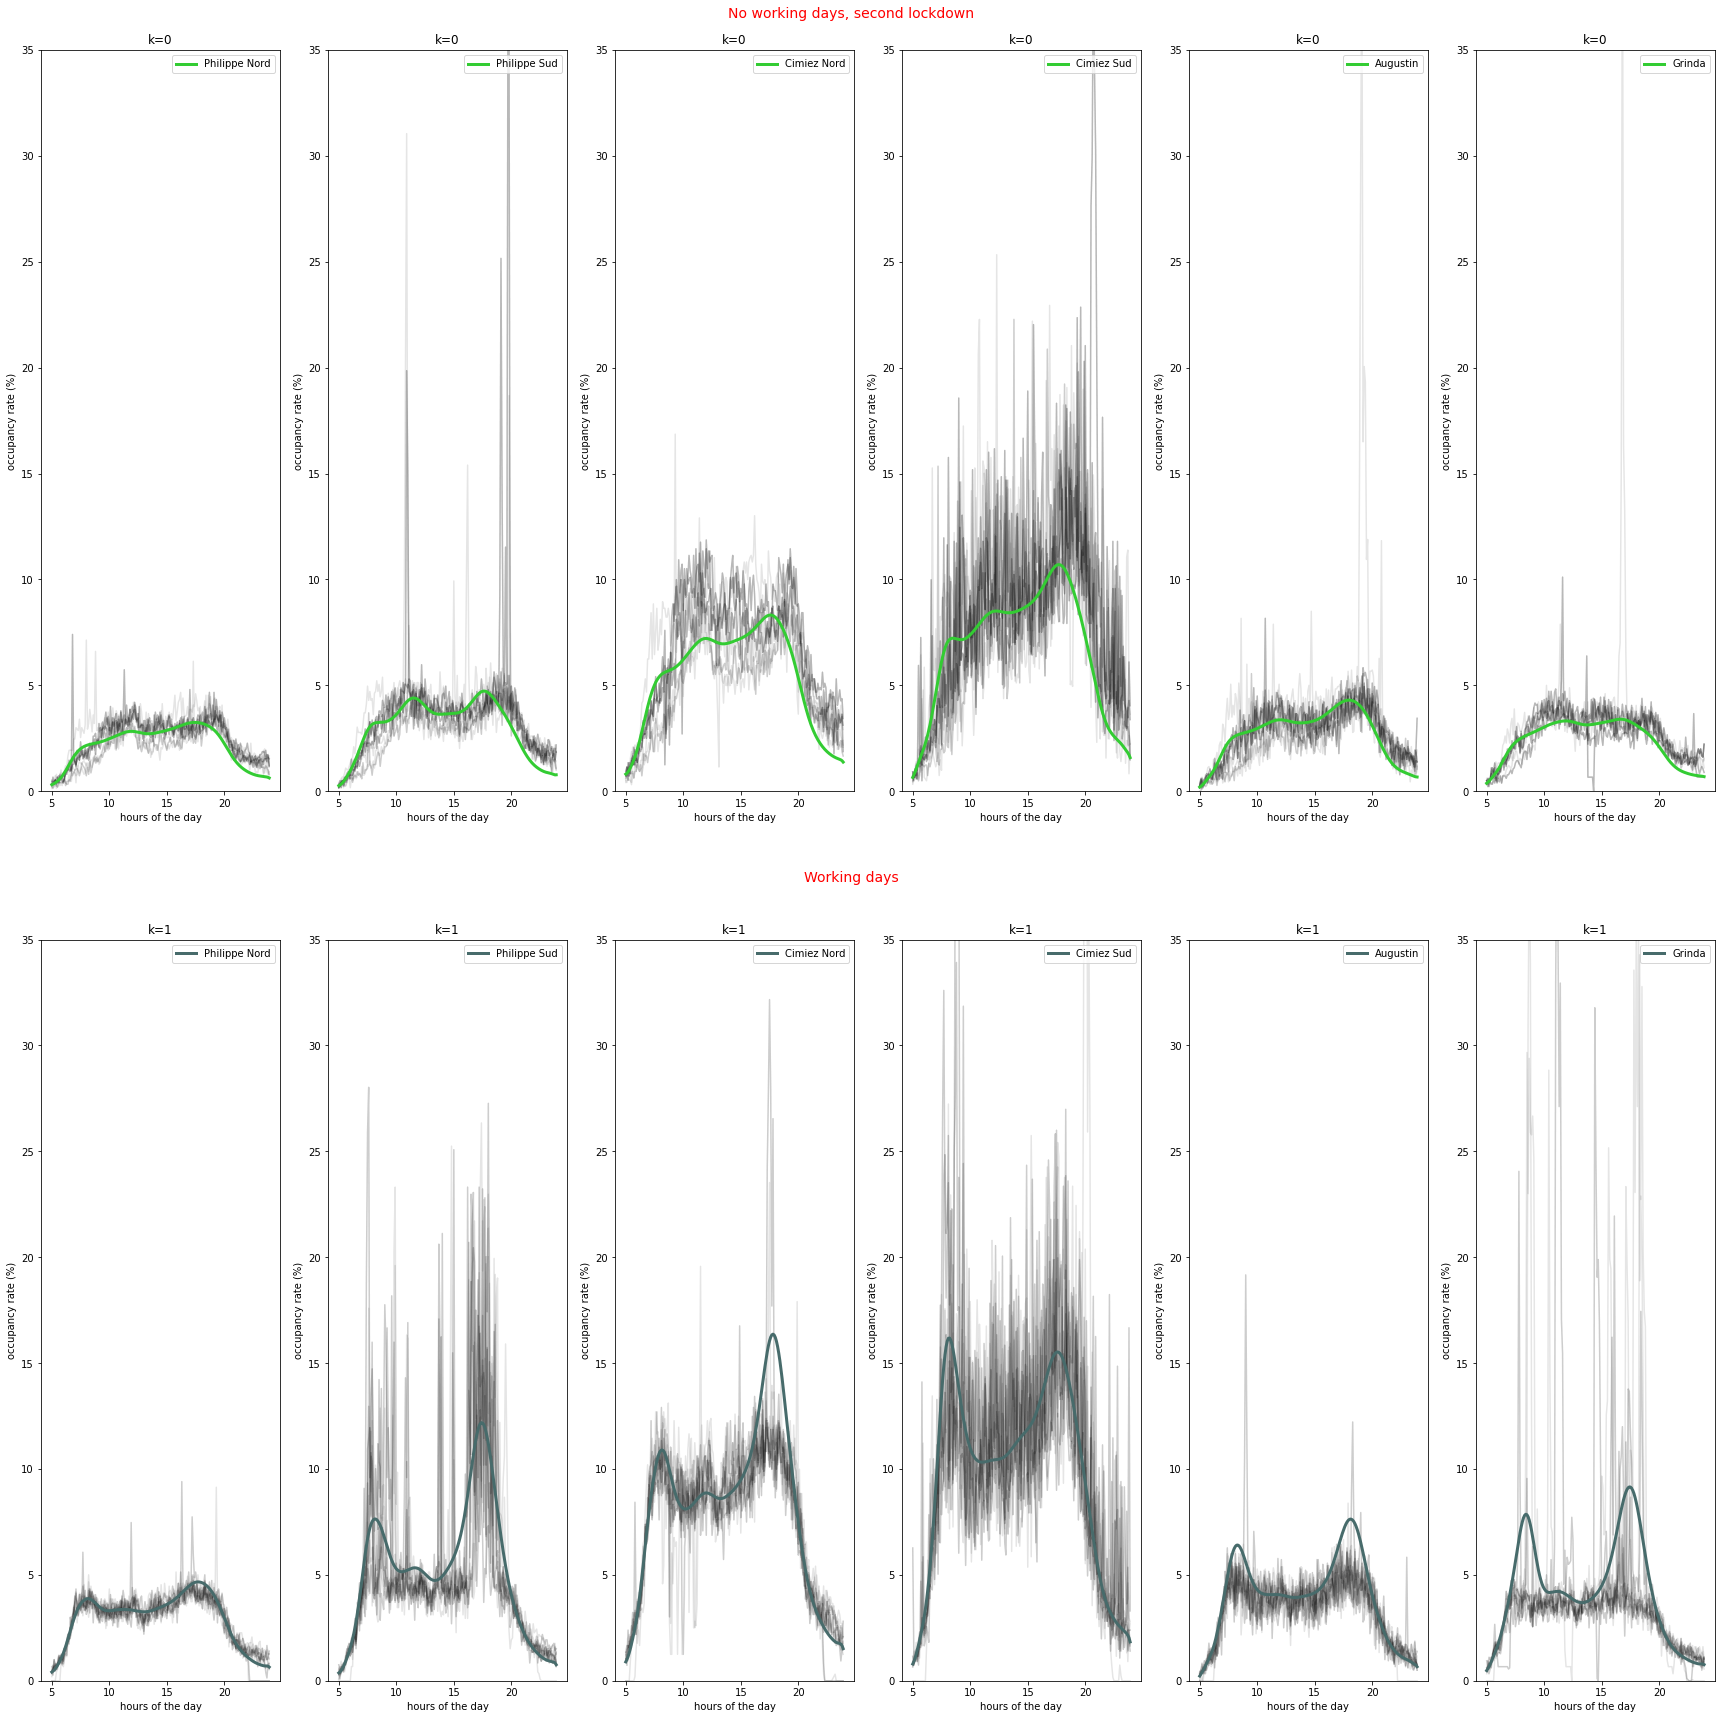
\includegraphics{centroids K=2 softDTW 2020.png}
    \caption{}
    \label{Fig 4.10}
\end{figure}

\emph{\small Figure 4.10 centroids of K-means, two clusters from 31/8/2020 to 31/12/2020}

    \hypertarget{conclusion}{%
\section{Conclusion}\label{conclusion}}

    Through this project, the softDTW seeded with K-means and GAK seeded
with Kernel K-means are proposed as clustering methods. Both softDTW and
GAK are proposed as alternative to the Euclidean distance and Dynamic
Time Warping. However, in literature is not yet explained if one method
is better than the other, hence the idea of use them together. Both
techniques used perform well in identify seasonal and daily paths of the
traffic. For Promenade the traffic detected by the airport detector
(C601) is different from the traffic detected by central located
detectors (C009/C094). Central located detectors show level of traffic
in the month of August different from the one registered by the airport
detector. In addition Thursdays and Fridays in the month of June,
September, October and December seem to be more trafficated in the night
hours, due to the proximity of central detectors to the City centre and
the sea. The shock on the traffic dynamic due to the first lockdown,
studied with Promenade data, reveals the dependency of the traffic to
the reopening of activities. For Voie Mathis due to the greatest amount
of usable detectors, two perspectives are proposed. To better identify
the days without ``school effect'', the aggregation of occupancy rate
time series of all detectors seems to have better result. The shock on
the traffic dynamic due to the second lockdown, studied with Voie Mathis
data, seems less prolonged in time with respect to the first one
analyzed with Promenade data.

    \section{Appendix} \label{Appendix}

    \subsection{ Promenade Des Anglais out of order detectors}

    \hypertarget{section}{%
\subsubsection{2019}\label{section}}

    \begin{itemize}
\item
  C602 detector: 4.32 \(\%\) of missing values for both flow and
  occupancy rate. No data from 19/8 from 6:00 to 8:54. No data from 29/8
  from 21:12 to 30/8 14:48. No data from 3/11 at 9:00 to 11:36. No data
  from 23/12 from 17:42 to 31/12.
\item
  C077 detector: 56.72 \(\%\) of missing values. No data registered from
  1/6 to 30/9 at 9:06.
\item
  C614: 7.05 \(\%\) of missing values. No data available from 4/6 to 6/6
  and from 21/8 to 3/9.
\item
  C615: 46.81 \(\%\) of missing values for the occupancy rate. No data
  registered from 1/6 to 30/9 at 9:06. 7.04 \(\%\) of missing values for
  the flow. No data registered from 4/6 at 17:00 to 6/6 at 15:00 and
  from 21/8 at 13:12 to 3/9 at 16:18 for the flow.
\item
  C599: 12.68 \(\%\) of missing values. No data available from 12/7 to
  15/7 and from 11/10 to 30/10.
\item
  C598: 64.39 \(\%\) of missing values for both flow and occupancy.
\end{itemize}

    \hypertarget{section}{%
\subsubsection{2020}\label{section}}

    \begin{itemize}
\item
  C615: 30.15 \(\%\) of missing values for the occupancy rate. No data
  registered for the occupancy from 6/4 to 21/6.
\item
  C077: 10.735 \(\%\) of missing values for both flow and occupancy. No
  data from 24/2 at 22:24 to 28/2 at 8:30. No data from 8/9 at 15:24 to
  10/9 at 9:48. No data from 12/9 at 13:06 to 16/9 at 14:42.
\item
  C598: 8.24 \(\%\) of missing values for both flow and occupancy. No
  data from 9/9 to 14/9 . No data from 3/10 to 6/10.
\end{itemize}

    \subsection{Voie Mathis out of order detectors}

    \hypertarget{section}{%
\subsubsection{2019}\label{section}}

    \begin{itemize}
\item
  Augustin: speed and occupancy abberrant data from 2/2 to 15/03.
\item
  Grinda: speed and occupancy abberant data from 2/2 to 15/03.
\item
  Philippe Sud: speed measurement are not reported for the entire year.
\end{itemize}

    \hypertarget{section}{%
\subsubsection{2020}\label{section}}

    \begin{itemize}
\item
  Gloria: for speed and occupancy problem of measurement starting from
  22/09 to 31/12.
\item
  Grinda: for speed and occupancy problem of measurement starting from
  04/01 to 08/01, from 14/04 to 20/04.
\item
  Magnan: for speed and occupancy problem of measurement starting from
  27/07 to 31/12.
\item
  Philippe Sud: speed measurement are not reported for the entire year.
\end{itemize}

    \bibliographystyle{unsrt}

\bibliography{ref}


    % Add a bibliography block to the postdoc
    
    
    
\end{document}
